\documentclass[journal, 11pt]{IEEEtran}

\usepackage{epsfig,rotating,setspace,latexsym,amsmath,epsf,amssymb,bm,amsbsy}
\usepackage{cite,graphicx,color,subfigure,here}
\usepackage{amsmath}
\usepackage[normalem]{ulem}
\usepackage{algorithm}
\usepackage[noend]{algpseudocode}
\usepackage{epstopdf}
\usepackage{scrextend}
\usepackage{ifpdf}
\usepackage{authblk}
\usepackage{caption2}
\usepackage{caption3}
\usepackage[english]{babel}
\usepackage{dsfont}
\usepackage{hyperref}
\providecommand{\keywords}[1]{\textbf{\textit{Index terms---}} #1}

\newcommand{\ba}{\begin{align}}
\newcommand{\ea}{\end{align}}


\begin{document}
\title{Connected Vehicles: Cognition Can Save Lives}

\author{Bengi Aygun$^\dag$, Mahni Shayganfar$^*$, and Alexander M.
Wyglinski$^\dag$\\
\normalsize $^\dag$Department of Electrical and Computer Engineering, Worcester
Polytechnic Institute, Worcester, MA\\
\normalsize $^*$Department of Computer Science, Worcester Polytechnic Institute,
Worcester, MA\\
\normalsize \{baygun, mshayganfar, alexw\}@wpi.edu}

\maketitle

\begin{abstract}
The idea of autonomous cars and connected vehicles is becoming increasingly
pervasive in research labs and car manufacturing companies. It is inevitable
that roads are going to accommodate autonomous and semi-autonomous vehicles
in the near future. However, like other technologies filtering into humans
daily life, the transition from conventional transportation systems to
autonomous vehicles requires careful involvement of human-oriented factors into
related technologies. We believe employing cognition in vehicular decision
making processes improves the awareness and consequently safety and comfort in
the roads. Here, we discuss how affect-driven integration of cognition into
connected vehicles can do so.
\end{abstract}

\begin{keywords}
Cognition, Awareness, Connected Vehicles.
\end{keywords}%

\IEEEpeerreviewmaketitle

\section{Become Connected, Become Aware}

In February~2014, the National Highway Traffic Safety Administration (NHTSA)
announced that Intelligent Transportation Systems (ITS), including connected
vehicle technology, will be required in all cars by 2019~\cite{factsheet}.
Subsequently, there has been a significant increase in research activities with
respect to vehicular networks (VANETs) in respond to this urgent need to
address vehicular traffic safety concerns~\cite{ntsb}. The information flow
within a connected vehicle network, which includes both vehicle-to-vehicle (V2V)
and vehicle-to-infrastructure (V2I), is managed via the broadcasting of control
messages over a control channel. In Europe, these messages are referred to as
Cooperative Awareness Messages (CAMs) while in the United States they are called
Basic Safety Messages (BSMs). Shared information, such as vehicle position,
motion characteristics, and vehicle size, are used for increasing the overall
environmental awareness in support of \textit{safety applications,}
(\textit{e.g.,} intersection movement assist, left turn assist, do not pass
warning sign, and light violation warning) as well as \textit{mobility
applications,} (\textit{e.g.,} collision warning, road coefficient of friction,
road conditions, parking management, and payment
solutions)~\cite{hardingNHTSA14}.

Semi and fully autonomous vehicles improve traffic safety by preventing
human-driver mistakes. Google and Ford are performing one of the mainstream
trials of autonomous vehicles while Volvo and Honda are working on increasing
vehicles' awareness through providing robust connectivity in vehicular
environments. Toyota Group recently announced that it is investing \$$50~M$ to
design and produce artificial intelligence within vehicular networks
~\cite{toyota50M}. Connected vehicles stand as a breakthrough in intelligent
transportation, while introducing some technological challenges. In order to
enable robust and efficient ITS mechanisms, several technical challenges
associated with autonomous vehicles must be addressed, including:

\begin{itemize}
\item Human-driver errors confront autonomous systems with unexpected
situations that make predefined decision mechanisms insufficient,
\item Dynamic vehicular environments include obstacles that vary with time,
changing number of vehicles, and varying road topology,
\item Decision making mechanisms in ITS are not delay-tolerant since the network
environment changes rapidly,
\item Frequently broadcasting between connected vehicles causes overhead on the
processing unit at each vehicle.
\end{itemize}

One promising feature that is under investigation in autonomous cars is
cognition. {\color{red} Cognition in vehicles is the functionality that
integrates vehicle's sensory information into several underlying mechanisms
enabling reasoning which subsequently improves safety and awareness in the
vehicles. This level of awareness impacts the interaction between the vehicle
and its occupants as well as the vehicle's control with respect to the
status of other neighboring vehicles. As a result,} cognition enables vehicles
to improve driving quality by improving safety of the vehicle's occupants and
other vehicles~\cite{cogcar}. Moreover, the driver or passenger's thoughts and
habits will be linked to decision processes. This feature provides a method to
transition from fully human driven to half autonomous and half human driven, and
finally to fully autonomous vehicles on roads.

We believe cognition in connected vehicles can:

\begin{itemize}
  \item reduce the amount of errors on the roads caused by drivers, since
  autonomous vehicles will not only drive based on more accurate perception, but
  will also include the behavior models of their neighbors before making any
  decision,
  \item reduce the amount of required communication since the autonomous cars
  only need to transfer high level decisions based on their own sensory
  information rather than an enormous amount of low level sensory data,
  \item improve the quality of travelling on the roads in terms of safety and
  comfort, since cognition increases awareness of each autonomous vehicle on the
  road.
\end{itemize} 

\section{Connected Vehicles and Driving Environments}

\subsection{Building Blocks of A Connected Vehicle}

Hardware components shape the technical practicality and readiness of ITS
solutions~\cite{hardingNHTSA14}. Our proposed cognition framework uses existing
components without requiring extra functionality. 

{\color{red}The intra-vehicle components, which are categorized in three main
blocks, and the autonomous vehicle testbed located in WPI Wireless Innovation
Laboratory are shown in Figure~\ref{fig:overall-prototype}.}

The intra-vehicle components
are categorized in six main blocks as shown in Figure~\ref{fig:invehComp}. As
shown, the internal vehicle components include two DSRC radios, which
standardization is still under development. One proposal is to dedicate one
radio permanently to safety messages. An alternative proposal is to design a
multi-channel hopping algorithm to use the radios adaptively. These radios
provide information sharing with other ITS members to increase awareness on the
roads.

\begin{figure}[ht]
  \subfigure[General Concept.]{
  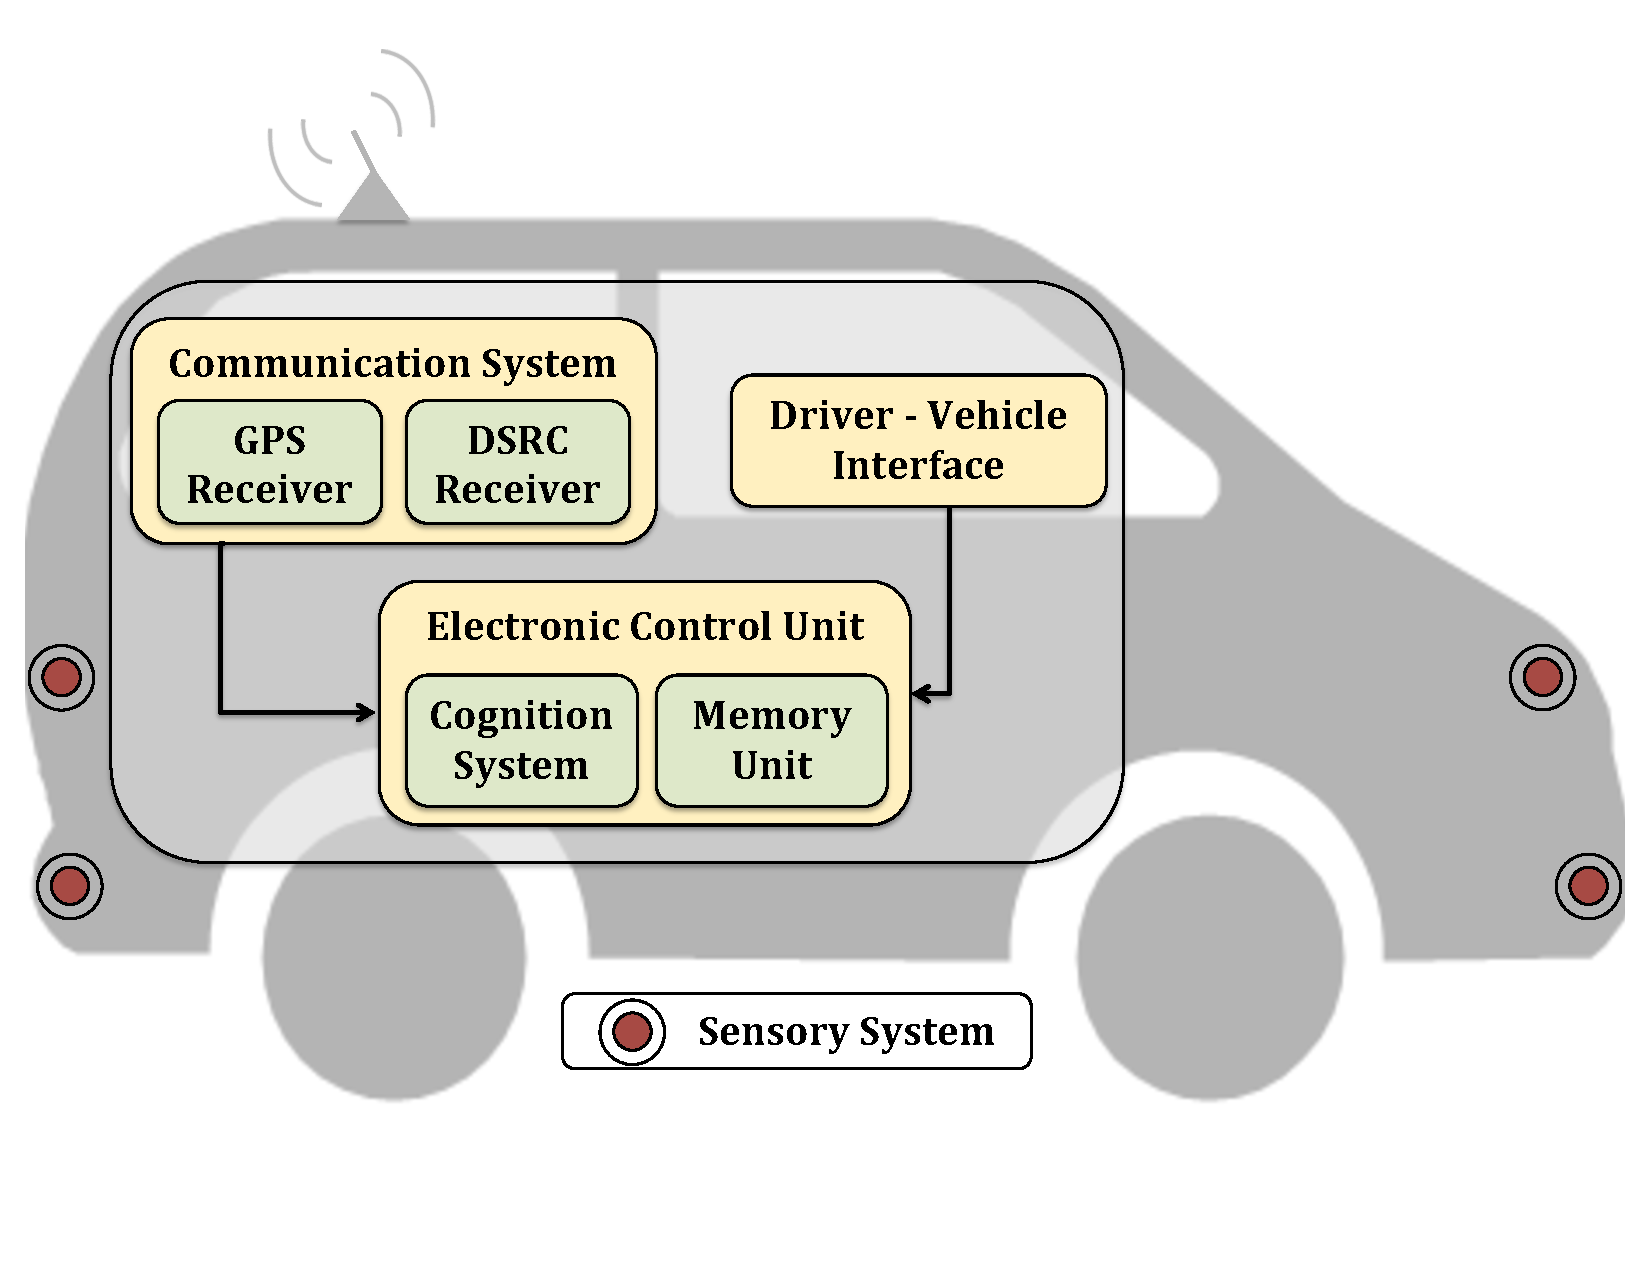
\includegraphics[width=0.48\textwidth]{figs/car.pdf}
  \label{fig:invehComp}}
  \quad
  \subfigure[Prototype System.]{
    \includegraphics[width=0.21\textwidth]{figs/front.pdf}
    \label{fig:prototype}}
  ~
  \subfigure[Server \& Radio Units.]{
  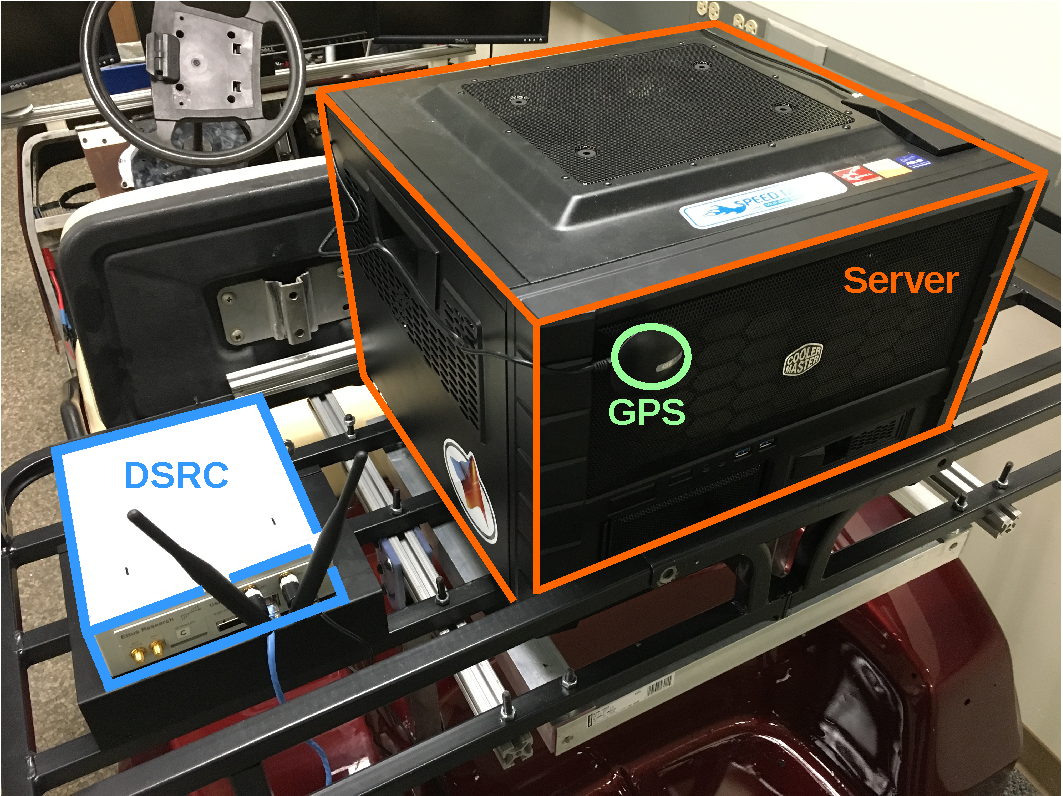
\includegraphics[width=0.23\textwidth]{figs/server.pdf}
  \label{fig:server}}
  ~
  \subfigure[User Interface.]{
  \includegraphics[width=0.47\textwidth]{figs/back.pdf}
  \label{fig:ui}}
  \vspace*{-4mm}
  \caption{Prototype of our autonomous vehicle}
  \label{fig:overall-prototype}
  \vspace*{-6mm}
\end{figure}

Another vital component for cognition in vehicles is the Global Positioning
System (GPS) receiver for gathering position and timekeeping information. A
computer processing unit uses this information with the data generated from
onboard sensors such as heading, speed, and acceleration to provide the
information to intra- and inter- vehicle intelligence systems. The safety
electronic control unit prepares BSMs to periodically broadcast in order to run
the safety applications. The memory unit satisfies the needs of the data
acquisition system and records the historical data on the cognition of its
own and other vehicles. The memory unit also stores security certificates.
Lastly, a driver-vehicle interface would issue warnings to the driver. Such
warnings could be audible, visual, or haptic, e.g., any type of audio-visual
alarm, tightening of the seat belt, or vibrating the driver's seat.

\subsection{Roads as Social Environments}

A social environment contains one's social relationships as well as one's
resources and physical surroundings. A social relationship is the most dynamic
part of a social environment. Hence, developing and maintaining positive social
relationships is crucial for a social environment and is influenced by the
individuals' quality of interaction. Roads are social environments in which
individual vehicles interact with each other through their ``nonverbal"
behaviors, each subject to the same traffic laws. However, there are many
violations of the laws on roads all over the world on a daily basis which
leads to expensive and all-too-often heart-breaking failures. These failures are
mostly caused by the failure of drivers to effectively interpret their driving
environment and make appropriate decisions with respect to their constraints
such as lack of time, lack of perception, and a plethora of cognitive load.
Therefore, it is crucial to involve cognition in the vehicles to share the
\textit{meaning} of what they perceive rather than broadcasting data coming
from their sensory system. For example, any sensory information leading to an
alert on a particular vehicle does not necessarily have the same meaning for
both the occupants and the neighbors of that vehicle. The alert warns the
occupants of the vehicle to be aware of an internal failure (e.g., malfunction
in the transmission system), or an external adversary (e.g., an animal
unexpectedly leaping into the road). The same alert has a different meaning
for a close vehicle approaching from behind; no matter what caused the alert
in the leading vehicle, the posterior vehicle should slow down effective
immediately. However, the same alert can be interpreted in an entirely different
way for a neighbor in front of the originally alerted vehicle. In fact, this
vehicle can ignore the received alert and continue a safe drive. Ultimately,
these type of improvements leads to a higher quality of vehicles' interaction
which consequently increases the safety of the roads.

\subsection{Driving Needs Pareto Optimal Decisions}

Cognitive architectures are used to solve high-dimensional multi-objective
tasks and to make proper decisions with respect to the dynamics of such
environments. Most of the time the real world problems possess a high level of
complexity due to the dynamism involved in the environment. A social environment
is an example of such complex environments. A social environment includes humans
as variety of sources making decisions independently but interrelated to each
other. Roads are social environments and driving is the social act of drivers'
behavior. It is clear that driving involves many decisions in which a driver
needs to maintain its own objectives while recognizing objectives of the others.

\begin{figure}[!t]
  \centering
  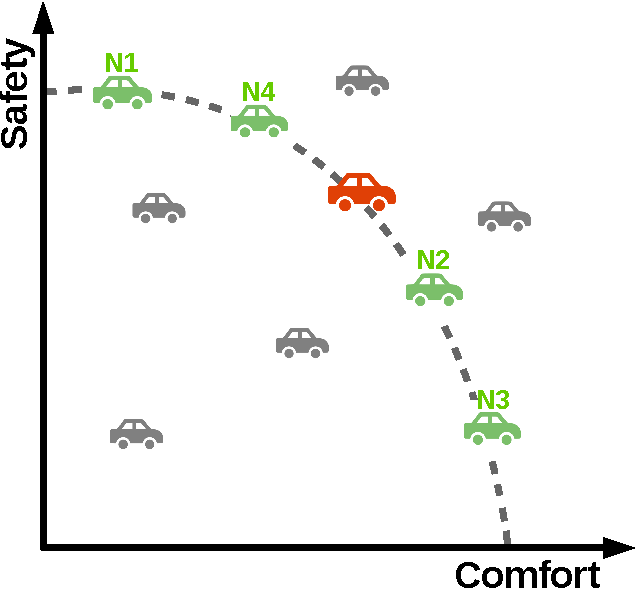
\includegraphics[width=0.35\textwidth]{figs/pareto-croped.pdf}
  \vspace*{-2mm}
  \caption{{\fontsize{10}{10}\selectfont Pareto optimal decisions for the
  neighbors.}}
  \label{fig:pareto}
  \vspace*{-6mm}
\end{figure}

Let's consider two general objectives, \textit{Safety} and \textit{Comfort}, for
any driver while driving between the source and the destination. Indeed, we can
expect all drivers would like to maximize both of these objectives. However,
while they need to obey the traffic law, they also need to take into account
their neighbors' driving behaviors, and respect their objectives. In the example
shown in Figure \ref{fig:pareto}, the red car's driver wants to maximize her own
safety and comfort to her aspiration level for both objectives to obtain the
``preferred'' point. We believe at least for a certain radius, the red vehicle
should consider objectives of the other vehicles in that neighborhood (four
vehicles shown in green), and update their anticipated and its own state based
on their behaviors. To achieve this goal, a cognitive system should be able to
make decisions such that it is impossible to make the state of self better
off without making the state of at least one of the neighbors worse off.
Therefore, the cognitive system's decision for any given event should be a
pareto optimal solution, since the neighboring connected vehicles' objectives
are important for each individual vehicle. Here, we only used the concept of
pareto optimality to discuss the type of decisions a cognitive system of a
vehicle should make. Our cognition framework and the underlying mechanisms do
not take a game theoretic approach to make decision-making.

\section{Cognition Systems}

Integration of cognition into connected vehicles needs us to understand the
building blocks of cognition, how they relate to each other, and what
functional operations they provide. We choose Newell's general theory of
cognitive control, PEACTIDM \cite{newell:unified-cognition}, to describe the
underlying abstract processes of a cognitive system. PEACTIDM is a theory of
cognitive control where cognition is decomposed into a set of eight abstract
functional operations \cite{newell:unified-cognition} all of which are
hypothesized as the building blocks of one's immediate behavior. Figure
\ref{fig:peactidm} shows the sequence of PEACTIDM's building blocks.

\textit{Perceive} is the reception of raw sensory data. For instance, connected
vehicles receive data from both their own local sensory system (e.g., GPS) and
their neighbor vehicles (e.g., an abrupt change in their velocities).
\textit{Encode} is the transformation of the sensory data into features that the
cognitive system can process. In the cognitive architectures using Bratman's BDI
paradigm \cite{bratman:intentions-plans} each sensory data will be transformed
into a new \textit{belief}. The cognitive architecture will be able to use these
beliefs in different processes. For example, in connected vehicles there will be
a belief about the current acceleration of the vehicle which corresponds to the
sensory data indicating this value. \textit{Attend} is the act of shifting or
maintaining the focus of attention on an event. For instance, an alert raised
because of a sudden speed reduction of multiple leading neighbor vehicles needs
to be attended to immediately, while the same alert does not need the same level
of attention if the leading vehicles are a few miles apart. \textit{Comprehend} is
the act of transforming an event into a goal or task-specific representation and
inferring the current status of the world. For instance, a vehicle receiving an
alert requiring an immediate reaction needs to identify the cause of the problem
even if the alert was raised and received from another vehicle. Thus, the
receiver of the alert can apply replanning if necessary.

\begin{figure}[!t]
  \centering
  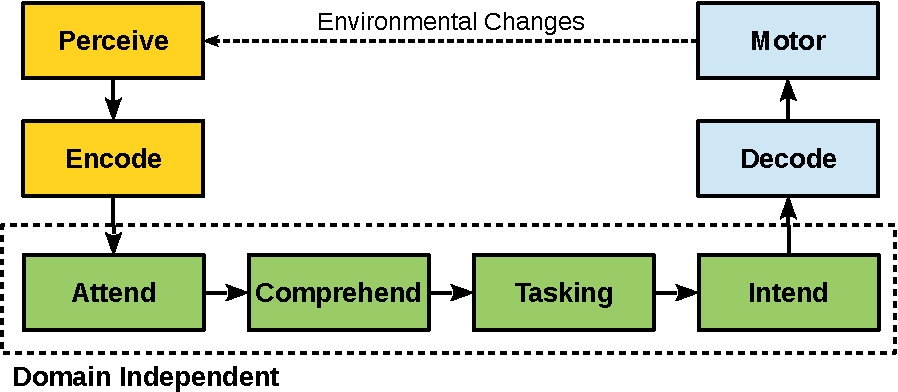
\includegraphics[width=0.485\textwidth]{figs/peactidm-croped.pdf}
  \caption{{\fontsize{10}{10}\selectfont PEACTIDM}}
  \label{fig:peactidm}
  \vspace*{-6mm}
\end{figure}

\textit{Tasking} is the process of recognizing a goal based on the new state of
the world. For example, a vehicle can recognize a goal in the plan to exit the
highway with respect to the new beliefs about an accident a few miles ahead and
the current state of the highway which includes slow-moving traffic.
\textit{Intend} initiates a future action based on the current goal as a
response to the current event. For instance, if the current goal of the vehicle
is to leave the highway, the vehicle begins to change lanes to the right-most
lane to be able to take the next exit. \textit{Decode} translates the response
based on the given \textit{intention} into a series of motor actions. For
instance, if the intention is changing lanes to the right, the vehicle applies a
series of actions including using the right blinker, checking the occupancy
status of the right lane, and turning the steering wheel to the right whenever
it is appropriate. \textit{Motor} executes the actions decoded based on the
given intention. For example, in the case of a lane change, the blinker starts
to blink and the wheels turn to the right respective to the amount of change at
the steering wheel.

{\color{red} In the next section, we introduce our cognitive theory in which our
focus is on affect-driven goal-oriented processes involved in cognition.
Although, there is not a one-to-one relationship between depicted functional
operations in Figure \ref{fig:peactidm} and the mechanisms in Figure
\ref{fig:cpm}, the mechanisms in Figure \ref{fig:cpm} conceptually provide
functionalities of the abstract functions in Figure \ref{fig:peactidm}.}

\section{{\fontsize{11.5}{9}\selectfont Affective Motivational Collaboration
Theory}}
\label{sec:amct}

\textit{Affective Motivational Collaboration Theory}
\cite{shayganfar:theory-overview} is about the interpretation and prediction of
observable behaviors in a dyadic collaborative interaction. Affective
Motivational Collaboration Theory specifies the processes involved in the
progress of a collaboration and how they impact the collaboration's underlying
structure. This theory is built on the foundations of the \textit{SharedPlans}
theory of collaboration \cite{grosz:plans-discourse} and the \textit{cognitive
appraisal} theory of emotions \cite{gratch:domain-independent}.

The theory focuses on the processes regulated by emotional states. It aims to
explain both rapid emotional reactions to events as well as slower, more
deliberative responses. The observable behaviors represent the outcome of
reactive and deliberative processes related to the interpretation of the self's
relationship to the collaborative environment. The reactive and deliberative
processes are triggered by two types of events: \textit{external} events, such
as the other's \textit{nonverbal behaviors} and \textit{primitive actions}, and
\textit{internal} events, comprising changes in the self's mental states, such
as belief formation and emotional changes.

Affective Motivational Collaboration Theory explains how emotions regulate the
underlying processes when these events occur during collaboration. This theory
elucidates the role of motives as goal-driven affect-regulated constructs with
which an agent can form new intentions to cope with internal and external
events. Therefore, a new motive can become a new intention and the self can take
a new action based on the new intention.  The focus of the underlying mechanisms
is on the ones depicted as mental processes in Figure \ref{fig:cpm} along with
the mental states.

\begin{figure}[!t]
  \centering
  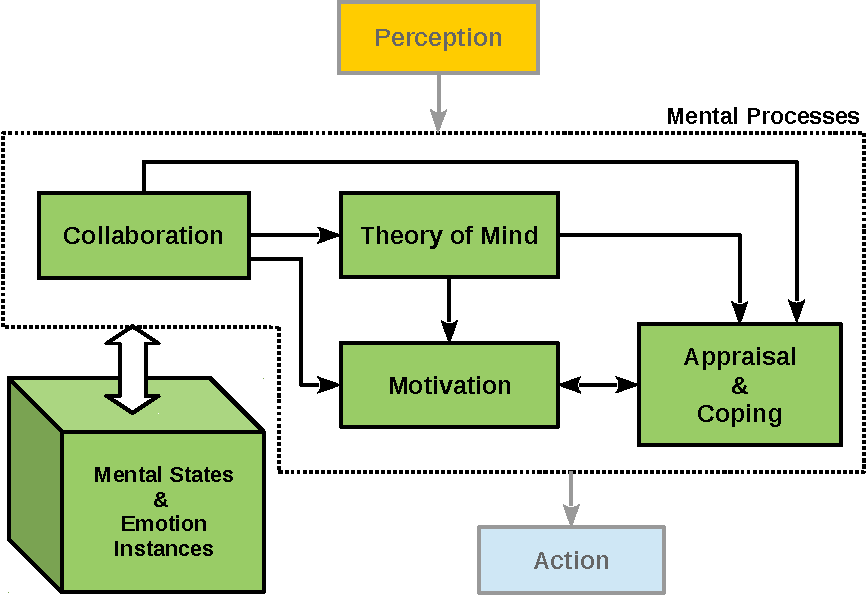
\includegraphics[width=0.485\textwidth]{figs/theory-general-croped.pdf}
  \caption{{\fontsize{10}{10}\selectfont Computational framework based on
  Affective Motivational Collaboration Theory (arrows indicate primary
  influences between mechanisms).}}
  \label{fig:cpm}
\end{figure}

The \textit{Mental States} includes ego vehicle's beliefs, intentions,
motives, goals and emotion instances as well as the anticipated Mental States of
the neighbors (other vehicles). For instance, every sensory data, every
threshold value, or every piece of inferred information about the world has a
corresponding belief in the Mental States. The \textit{Collaboration} mechanism
maintains constraints on actions, including task states and the ordering of
tasks. Although maintaining safety and comfort is a goal for each individual
vehicle, all vehicles also have a shared goal which is sharing the road with
others -- at least partially -- to get to their destinations. Therefore,
vehicles require the collaboration mechanism to maintain their full or partial
shared plan. The \textit{Collaboration} mechanism also provides processes to
update and monitor the shared plan. The \textit{Appraisal} mechanism is
responsible for evaluating changes in the ego vehicle's Mental States, the
anticipated Mental States of the neighbors, and the state of the collaboration
environment \cite{shayganfar:appraisal-short}. The outcome of appraisal impacts
every vehicle as an evaluative, regulatory, or motivative process. For instance,
the \textit{expectedness} of an event indicates how prepared the ego vehicle is
to cope with the event, or how to maintain the current state with respect to the
current changes in neighbors' location. The \textit{Coping} mechanism provides
the ego vehicle with different coping strategies associated with changes in the
ego vehicle's mental states with respect to the state of the collaboration. For
instance, does ego vehicle need to change speed with respect to the current
state of the road, or does it need to replan to get to the destination. The
\textit{Motivation} mechanism operates whenever the ego vehicle a) requires a
new motive to form a new intention with respect to the current event, or b)
wants to interpret a neighbor's motive whenever the neighbor's behavior triggers
an alarm after ego vehicle appraises the situation. The \textit{Theory of Mind}
mechanism is the mechanism that infers a model of the neighbor's anticipated
mental state. The ego progressively updates this model during the collaboration.
A neighbor's model impacts ego vehicle's decision with respect to the state of
the neighbor.

\section{Example Scenario}
\label{sec:example-scenario}

According to analysis of lane changes by the US' National Highway Traffic
Safety Administration (NHTSA) in 2003 \cite{nhtsa:lane-change} more than
38\% of pre-crash movements in the highways were caused by typical lane changes.
Furthermore, according to the NHTSA's traffic safety facts of February 2015
\cite{nhtsa:crash-stats}, about the 94\% of the critical reasons of
pre-crash events are attributed to the drivers. As mentioned in this report,
about 41\% of the driver-related critical reasons are because of the
\textit{\textbf{drivers' recognition errors}} including drivers' inattention,
internal and external distractions, and inadequate surveillance. Also, about
33\% of pre-crash reasons are caused by the \textit{\textbf{drivers' decision
errors}} such as driving too fast for conditions, too fast for the curve, false
assumption of others’ actions, illegal maneuver and misjudgment of gap or
others’ speed. In our hypothetical example, we show how the involvement of
different mechanisms in our framework can improve safety and comfort for both
the ego vehicle and the other neighbor(s) in the roads for such conditions.

\begin{figure*}[!t]
  \begin{center}
  \subfigure[Being aware of other drivers' intention.]{\label{fig:example1}
  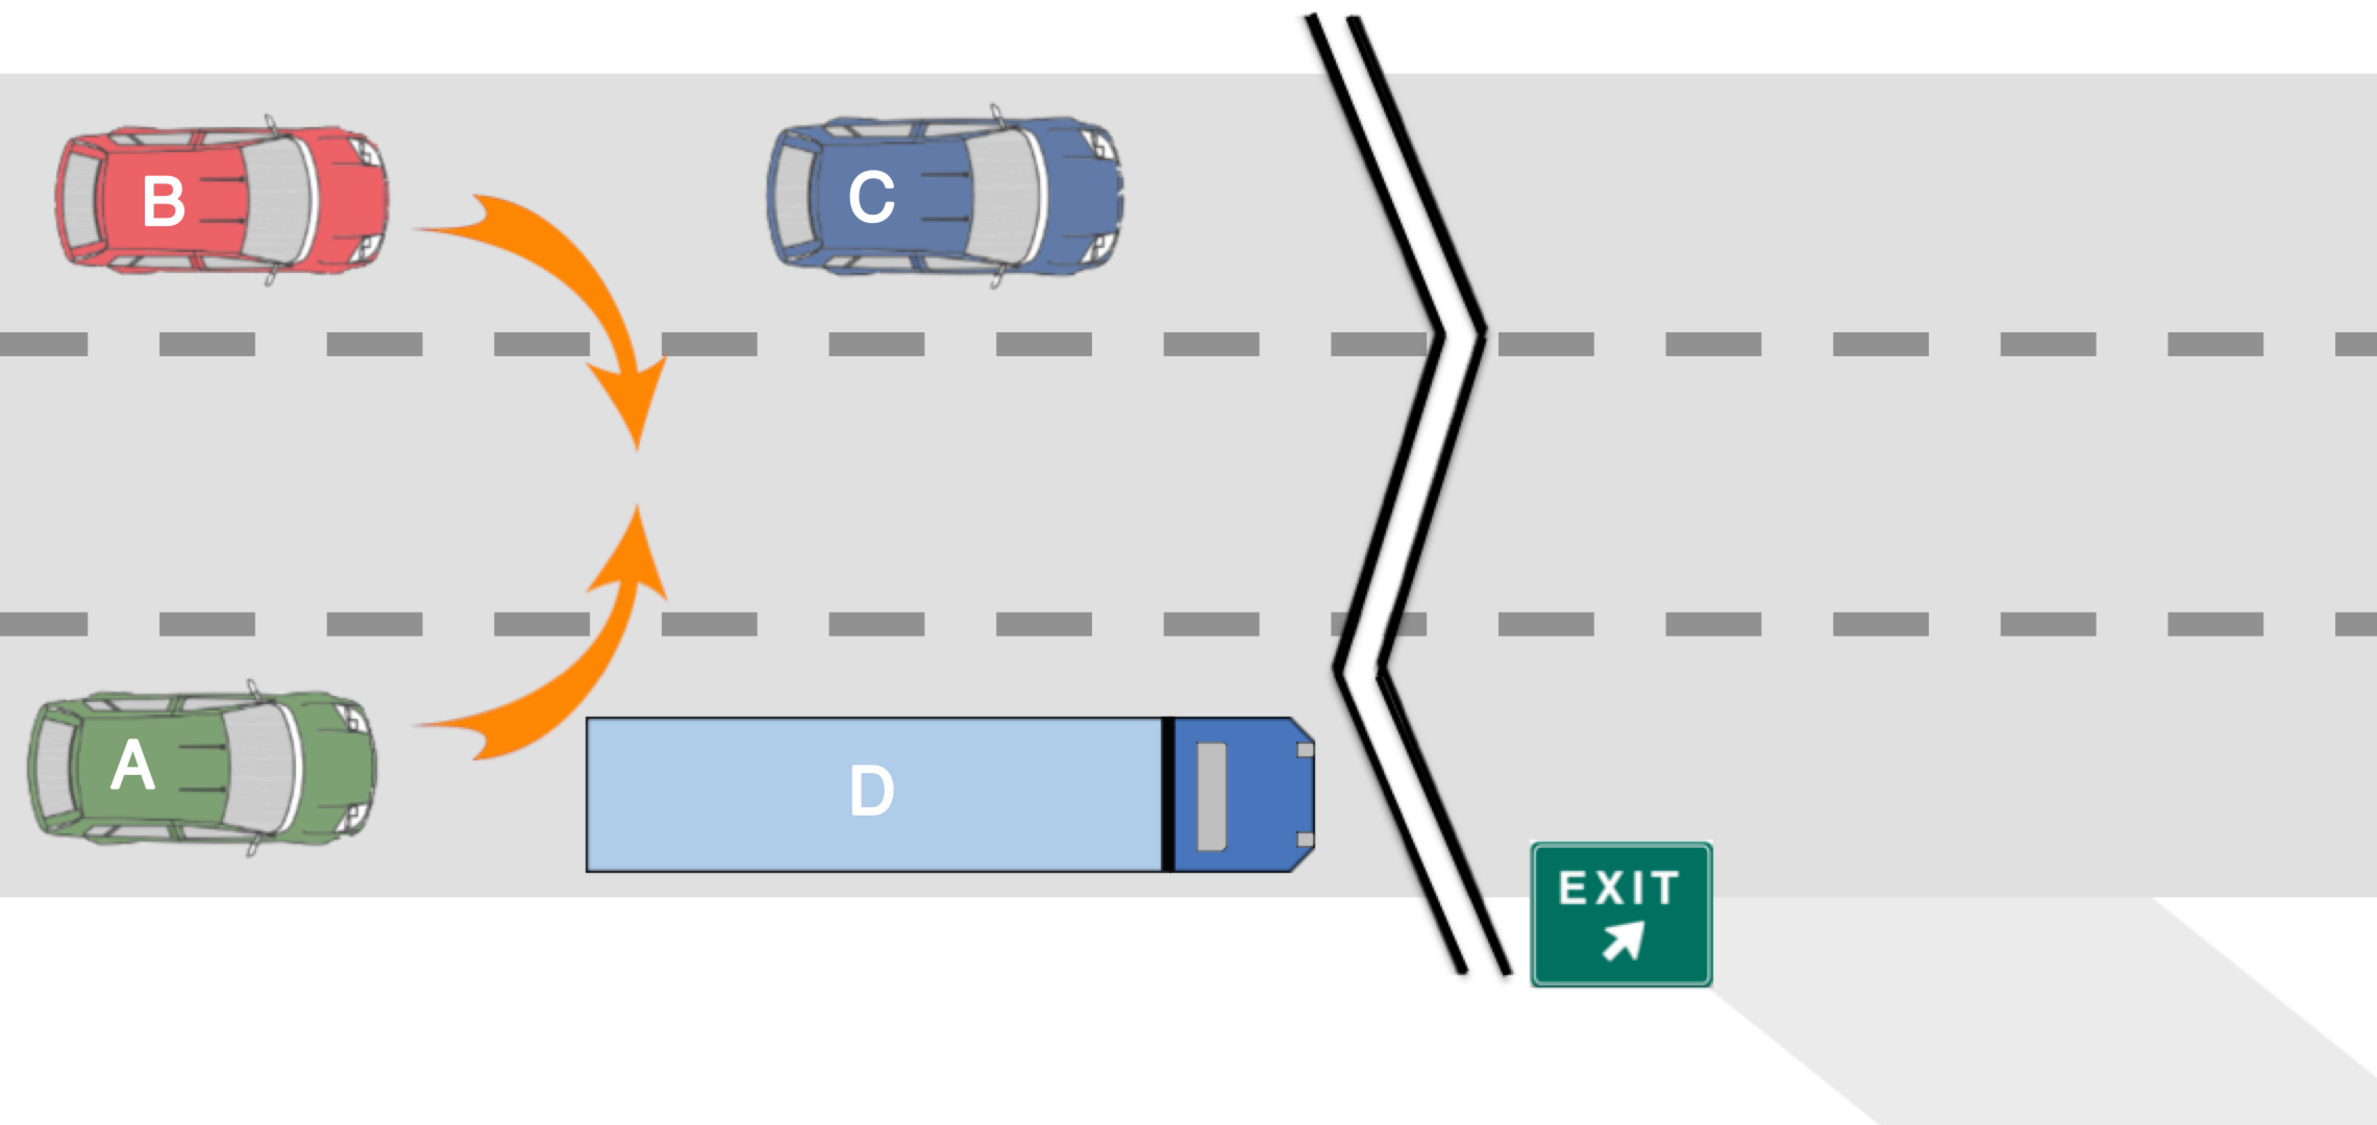
\includegraphics[width=0.55\textwidth]{figs/ex1.pdf}} 
  \subfigure[Coping with the driving behavior of a reckless
  driver.]{\label{fig:example2}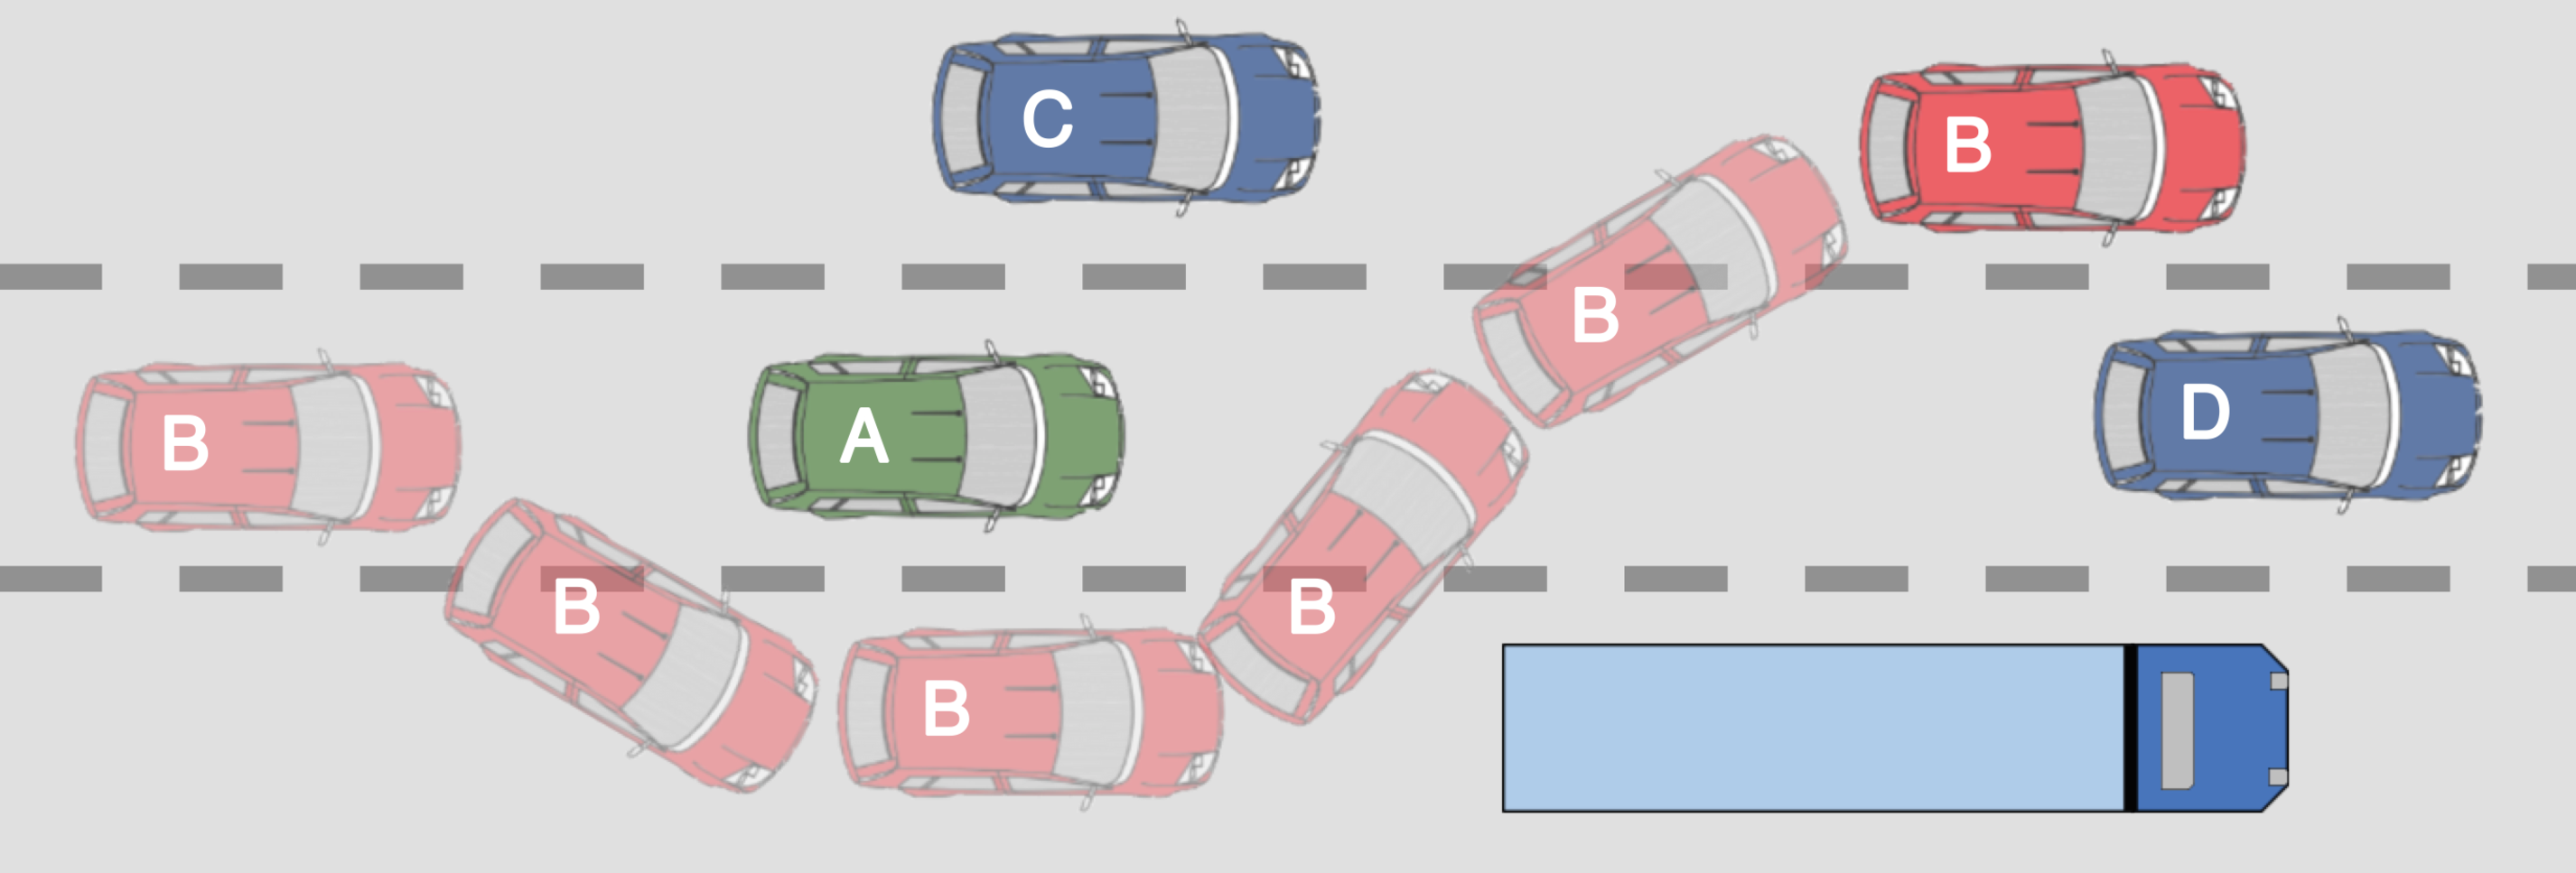
\includegraphics[width=0.55\textwidth]{figs/ex2.pdf}}
  \subfigure[Communicating the behavior model of careless
  driver.]{\label{fig:example3}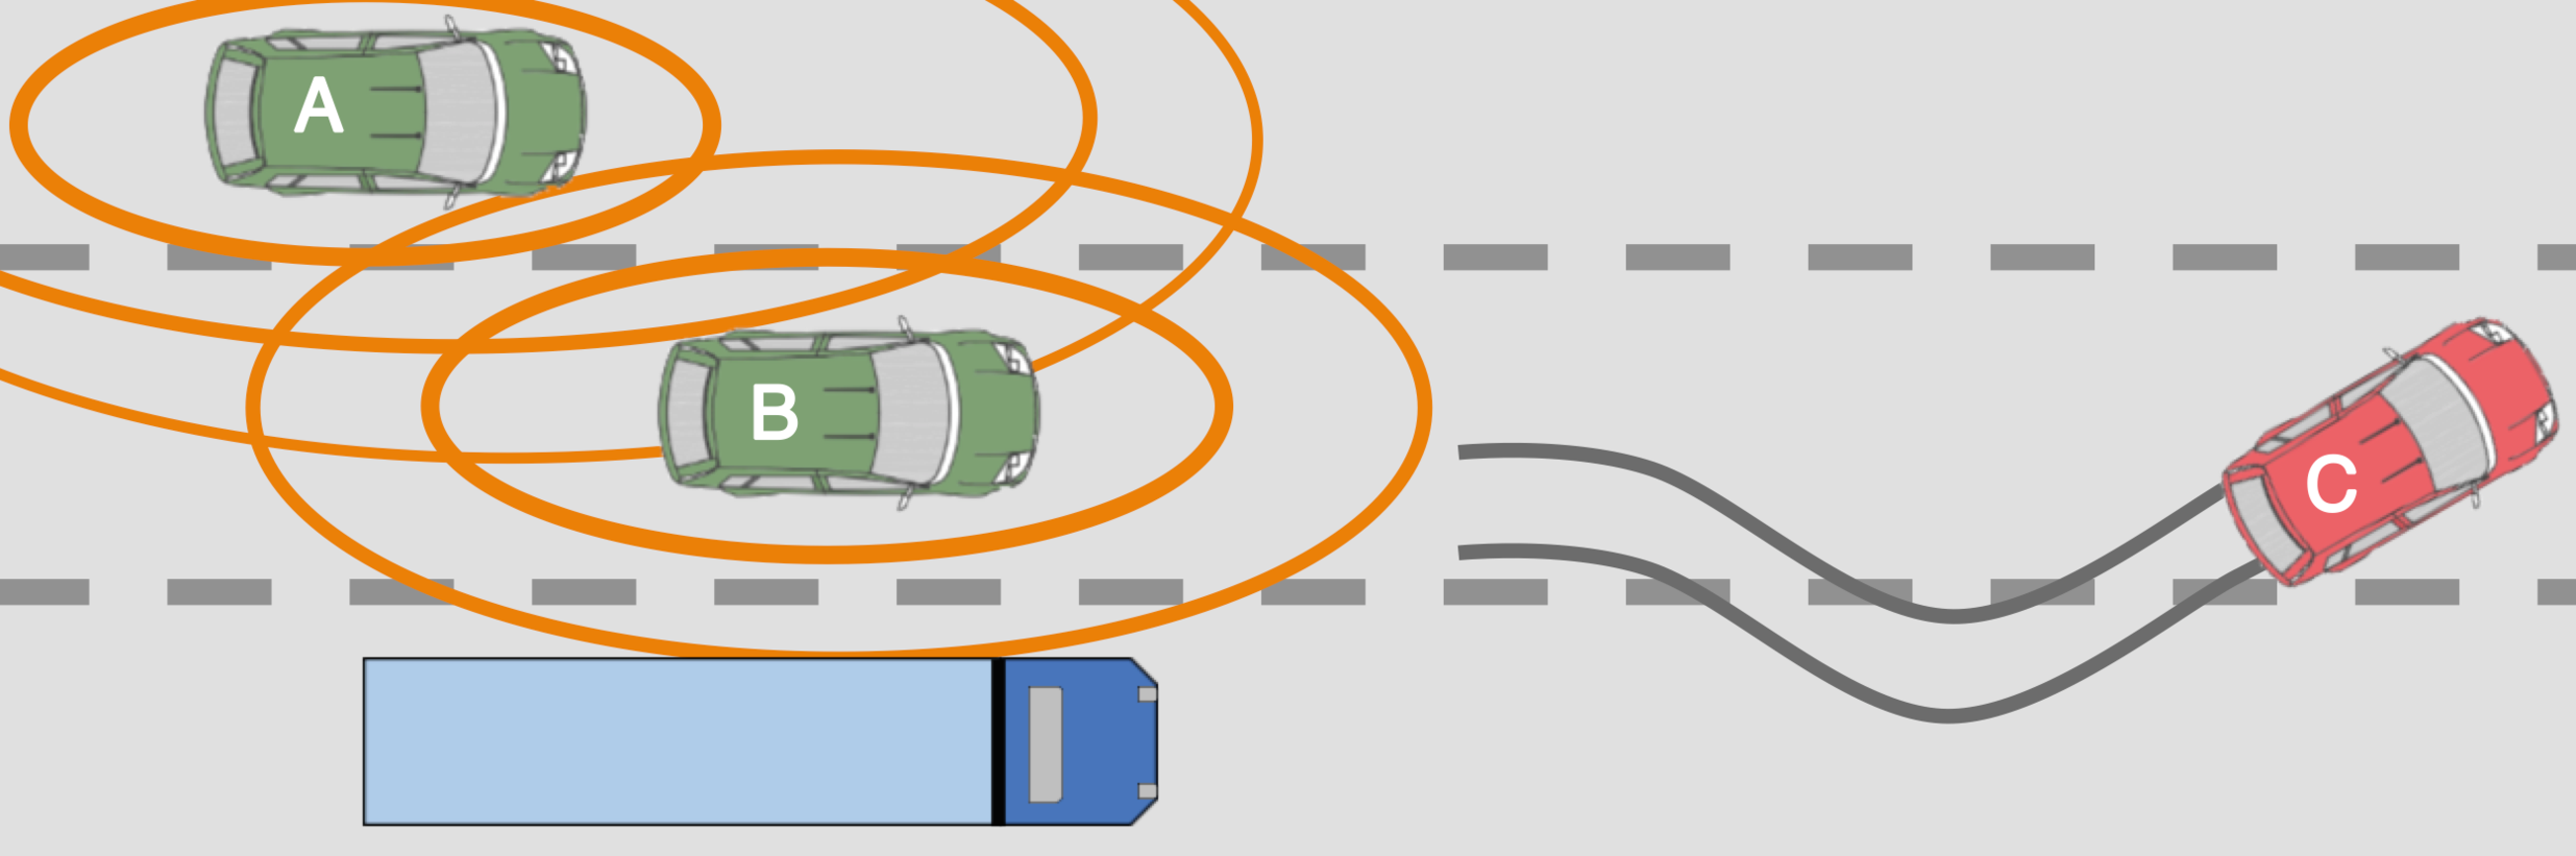
\includegraphics[width=0.55\textwidth]{figs/ex3.pdf}}
  \caption{Three incidents in our scenario.}  
  \label{fig:threeScenarios}
  \end{center}
\end{figure*}

In this example (see Figure \ref{fig:example1}), autonomous Vehicle \textit{A}
(ego vehicle) travelling in the right lane wants to take Exit \textit{x} in two
miles. However, the ego vehicle has decided to pass the slow-moving Truck
\textit{D} before taking Exit \textit{x}. At the same time, Vehicle \textit{B},
travelling in the left lane, quickly approaches a slower car, Vehicle \textit{C}
in the same lane. Vehicle \textit{B}'s driver decides to change lanes to the
middle lane to pass Vehicle \textit{C}. Therefore, both the autonomous Vehicle
\textit{A} and the driver of Vehicle \textit{B} want to go to the middle lane at
the same time; since the middle lane is not occupied by any other vehicle.
Hence, because both Vehicle \textit{A} and Vehicle \textit{B} are not aware of
each other's intention, they can cause an accident irrespective of the
responsibility of each vehicle with respect to the traffic law.

In this example, the ego vehicle perceives a sudden change of lane by Vehicle
\textit{B}; then it appraises this event as \textit{relevant, undesirable,
unexpected}, and \textit{controllable}. The lane change by Vehicle \textit{B} is
relevant to ego vehicle since it decreases the utility of the current goal for
the ego vehicle; it is undesirable since the ego vehicle's attempted goal (lane
change) is not achieved (i.e., it is blocked); it is unexpected since Vehicle
\textit{B} interrupted the ego vehicle's pursuit of its current goal; and it is
controllable since the ego vehicle still has three alternative goals.
The goal management process in our framework ranks all of the potential goals
based on their status in the plan structure, and the outcome of the self and the
reverse appraisal \cite{shayganfar:goal-management}. Moreover, in this incident
the ego vehicle does not have a behavior model of the Vehicle \textit{B}, since
Vehicle \textit{B} has just reached the ego vehicle and is perceived for the
first time. Therefore, first, the ego vehicle replaces the current goal with
stay-in-the-lane goal for the purpose of recovering from the blocked goal. In
general, the ego vehicle adopts one of the safe predefined tactical goals, e.g.,
stay-in-the-lane or reduce-speed, as an alternative goal to the original goal
which would raise unexpected and undesirable events. Next, the ego vehicle
chooses the \textit{restraint coping strategy} to immediately pull back into the
right lane to yield the the middle lane to Vehicle \textit{B} avoiding any
possible accident. Therefore, choosing an appropriate coping strategy, the ego
vehicle responds to the current goal change using the sensory system and taking
appropriate actions to pursue the new stay-in-the-lane goal. The ego vehicle
updates Vehicle \textit{B}'s user model to a reckless driver. As shown in this
example, the cognition of the autonomous vehicle prevented an accident which
could happen because of the drivers' recognition error caused by their
inadequate surveillance of the highway.

In the next incident (see Figure \ref{fig:example2}), the ego vehicle perceives
Vehicle \textit{B} quickly approaching from behind in the middle lane (event 1).
Vehicle \textit{B} changes its lane to the right lane (instead of left) to pass
the ego vehicle immediately after reaching the ego vehicle (event 2). As
shown in Figure \ref{fig:example2}, Vehicle \textit{B} has to switch back to the
middle lane quickly (event 3), since there is a slow-moving truck in the right
lane at a short distance ahead of the ego vehicle. However, Vehicle \textit{D}
makes another blockage for Vehicle \textit{B} in the middle lane. Consequently,
Vehicle \textit{B} has to switch to the left lane to pass this blockage (event
4). All these four events happen in a few seconds in the neighborhood of the ego
vehicle.

\begin{figure*}
  \centering
  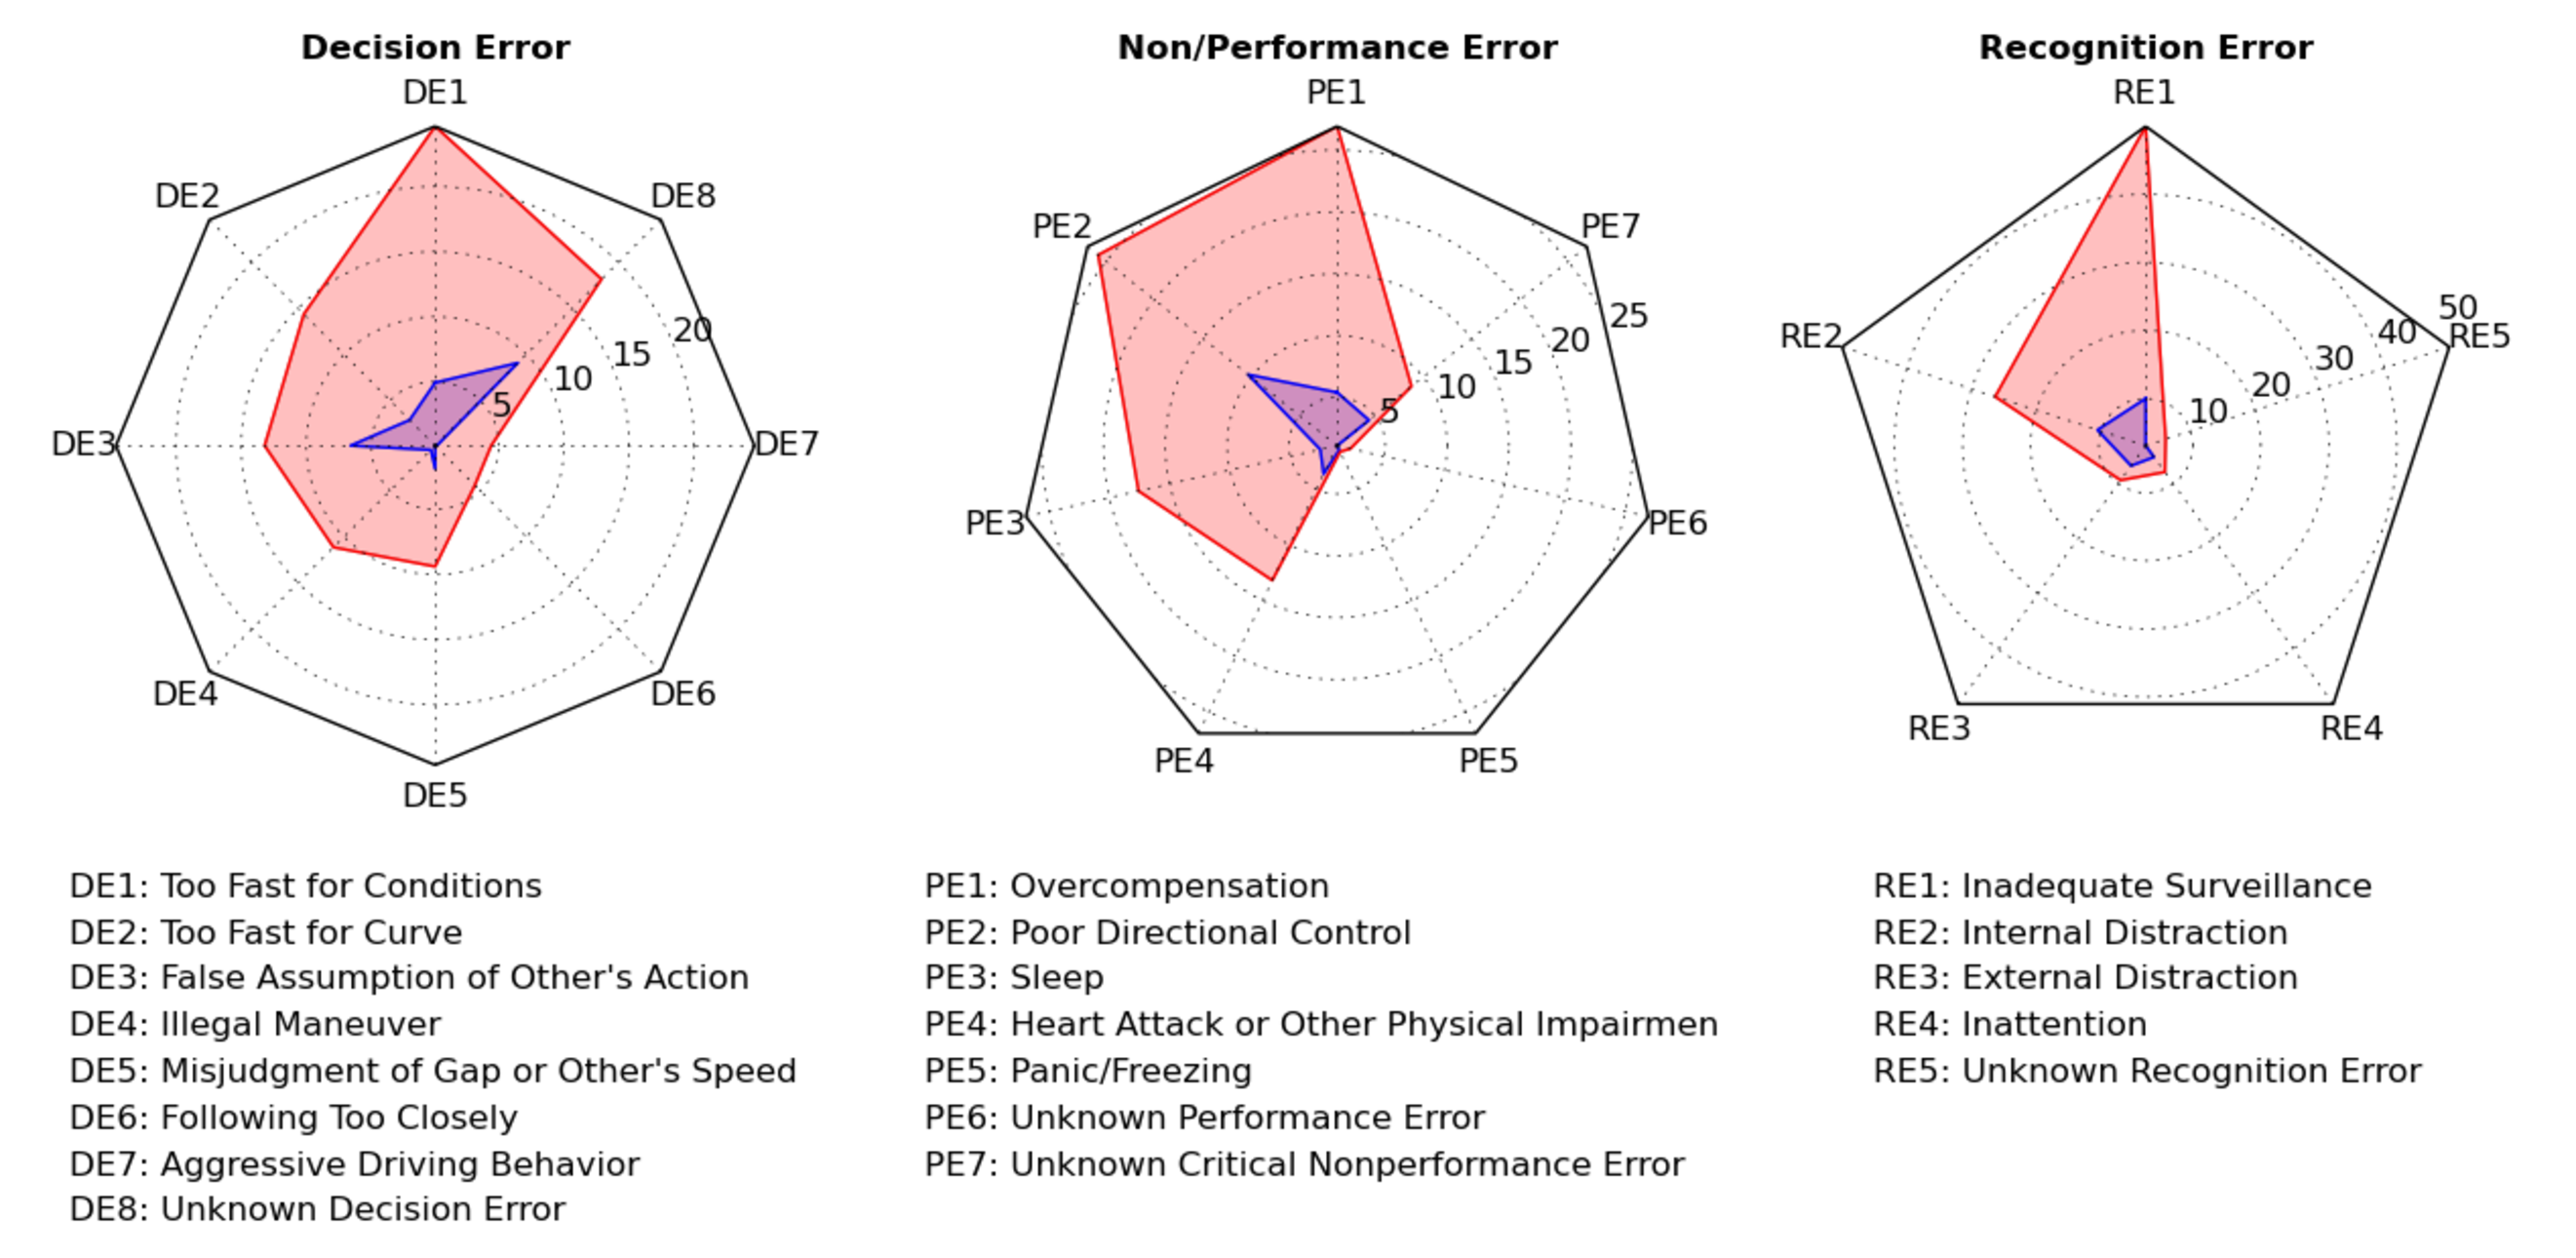
\includegraphics[width=\textwidth]{figs/CrashCriticalReasons.pdf}
  \caption{{\fontsize{10}{10}\selectfont Comparison of critical reasons for
  pre-crash events showing reduction in crashes, from conventional vehicles
  \cite{nhtsa:crash-causation} (red) to vehicles with cognition (blue),
  caused by Decision Error (left), Performance or Non-Performance Error
  (middle) and Recognition Error (right).}}
  \label{fig:errorPlot}
  \vspace*{-6mm}
\end{figure*}

Similar to the first incident, the ego vehicle appraises the first event as
highly \textit{relevant, undesirable, unexpected} and \textit{controllable} for
the self, and \textit{relevant, desirable} and \textit{expected} with low value
of \textit{controllability} for Vehicle \textit{B}. Therefore, the ego Vehicle,
creates a behavior model for Vehicle \textit{B} with a high probability of
having a \textit{speeding} driver. The next three events will be also appraised
in the same way. The ego vehicle updates Vehicle \textit{B}'s behavior model
based on each event, raising the probability of Vehicle \textit{B} having a
\textit{speeding} driver. Updating Vehicle \textit{B}'s behavior model based on
several events leads to a more accurate behavior model of Vehicle \textit{B}.
Consequently, the ego vehicle will able be to evaluate Vehicle \textit{B}'s
actions more accurately based on the reverse appraisal process. The outcome of
the self and reverse appraisal processes causes the goal management process to
employ another tactical goal, i.e., reduce-speed. Hence, the ego vehicle as the
outcome of the appraisal and the behavior modeling processes adopts
\textit{behavioral disengagement} as the most appropriate coping strategy.
Furthermore, Vehicle \textit{B}'s behavior model not only helps the ego vehicle
to be safe while travelling in its neighborhood, but it can also inform other
autonomous vehicles to drive carefully while Vehicle \textit{B} is within a
short distance from them.

In the last incident the ego vehicle (Vehicle \textit{A}) simply passes another
autonomous car (Vehicle \textit{B}) which is driving in the middle lane with a
normal speed (see Figure \ref{fig:example3}). Vehicle \textit{B} also detects
the appearance of another autonomous vehicle in its own neighborhood. The ego
vehicle receives an alert from Vehicle \textit{B} regarding the car (Vehicle
\textit{C}) travelling a few hundred feet in front of them in the middle lane.
The alert message contains a vector of probabilities of Vehicle \textit{C}'s
driver type indicating the following probabilities: 34\% chance of being
\textit{drowsy driver}, 32\% of chance of driving \textit{under the influence of
drugs or alcohol}, 28\% chance of being a \textit{distracted driver}, and 6\%
chance of being a \textit{teenage driver}. These values are computed by 
Vehicle \textit{B}'s Bayesian behavior modelling process in the the Theory of
Mind mechanism. The computation of these probability values is based on Vehicle
\textit{B}'s perception and appraisal of the road including Vehicle \textit{C},
even before the ego vehicle reaches to Vehicle \textit{B}. Afterwards, the ego
vehicle uses the content of alert message to update it's own behavior model
of the Vehicle \textit{C}. Updating Vehicle \textit{C}'s behavior model does not
change the ego vehicle's current goal. It also does not demand the ego vehicle
to apply an immediate reactive change in its own driving behavior. However, it
replaces the current motive (i.e., maintain the current speed) of the ego
vehicle with a new motive (i.e., maintain the current distance with Vehicle
\textit{C}). Forming this new motive is based on the outcome of the Theory of
Mind (updated by another vehicle) and the Appraisal mechanisms. The new motive
is urgent since it requires an immediate change in ego vehicle's driving
behavior, and it is important since it is related to the current goal that the
ego vehicle pursues. Therefore, the new motive causes the ego vehicle to adopt
an \textit{active coping strategy} to circumvent the stressor (i.e., Vehicle
\textit{C}) by maintaining its distance.

\section{Hypothetical Performance Results}

Recent reports show that traffic density and crash rate is highly correlated.
In~\cite{trb12}, the relationships between traffic density, speed and crash rate
are modeled based on traffic reports from Denver, Colorado. 

{\color{red}In Figure~\ref{fig:errorPlot}, the crash rate of Route I-70, Denver
is shown in the blue line in Winter 2012 at weekends based on annual traffic
report~\cite{trb12}. The crash rate is computed as the proportion of  the total
number of located crashes to the vehicle miles traveled on the corresponding
route. The crash types are defined in 37 categories in NHTSA Technical Report
released in 2014. The proposed cognition framework can prevent 26 - 34 of  these
crash scenarios by avoiding human-driven mistakes. While most of the crash
scenarios are avoided, some scenarios may or may not be eliminated based on
neighbor vehicle existence. Few crash scenarios caused by mechanical issues such
as vehicle failure cannot be prevented by the proposed cognition system. These
statistics summarized in Figure~\ref{fig:errorPlot} in red line indicates a
significant influence of using our proposed cognition framework, reducing the
crash rate based on the same data.}

\begin{figure}[!t]
  \centering
  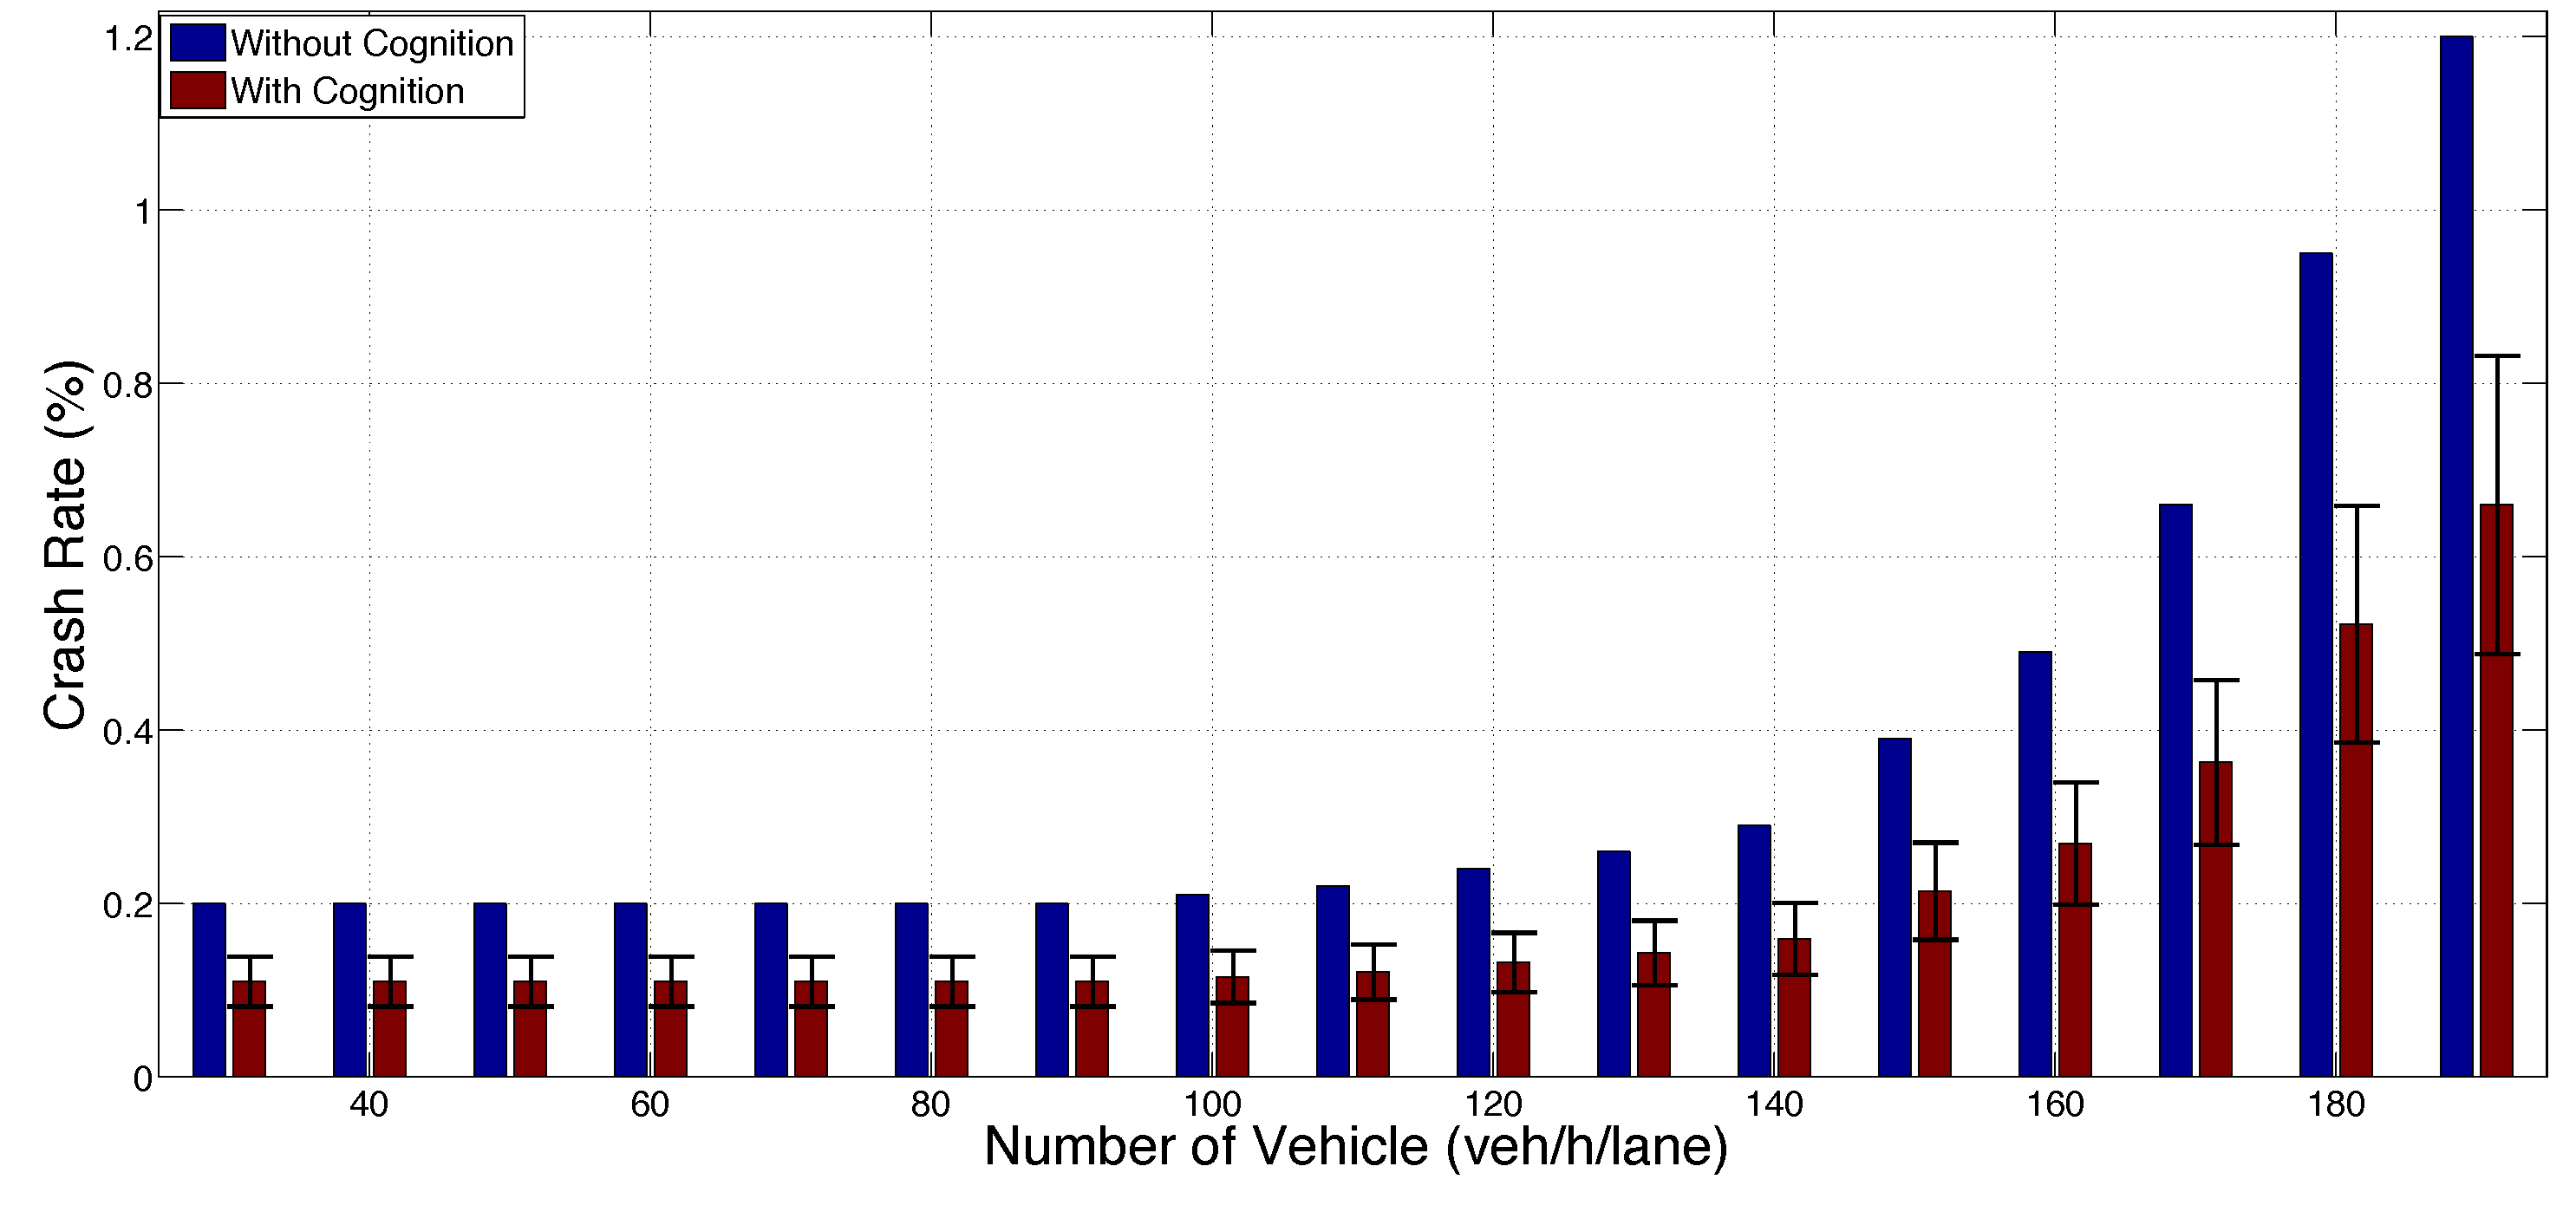
\includegraphics[width=0.49\textwidth]{figs/errorPlot.pdf}
  \caption{{\fontsize{10}{10}\selectfont The impact of cognition on reducing the
  crash rate caused by human error.}}
  \label{fig:errorPlot}
  \vspace*{-6mm}
\end{figure}

\begin{figure*}[!t]
  \begin{center}
  \subfigure[Urban Scenario.]{\label{fig:urbanVsTime}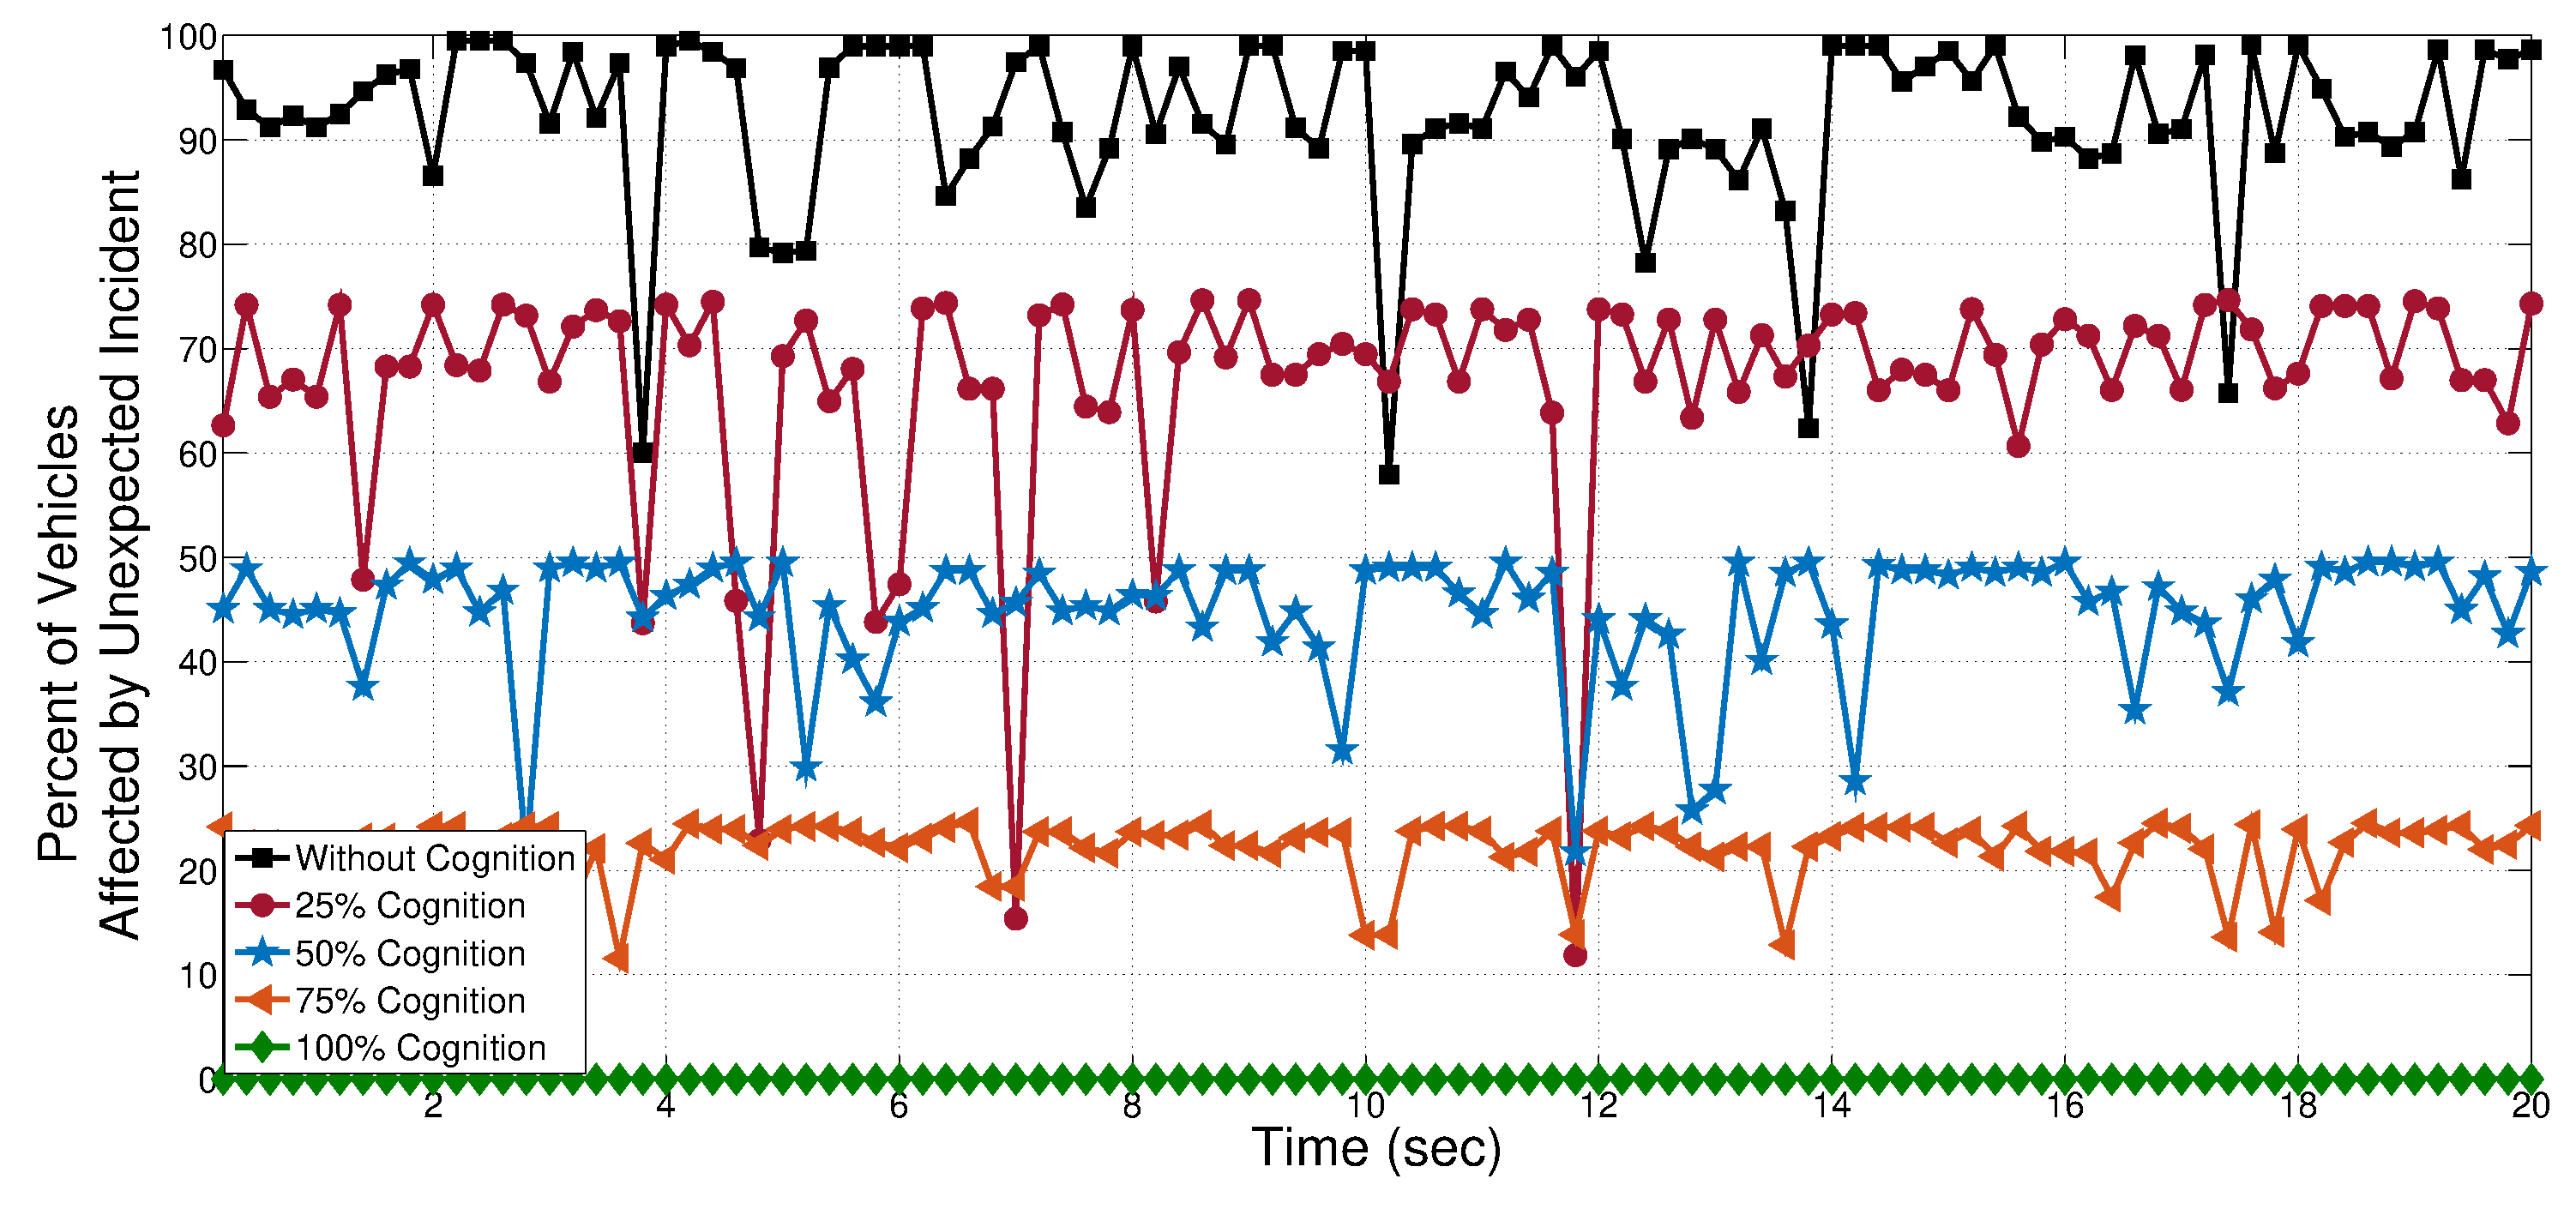
\includegraphics[width=0.45\textwidth]{figs/urbanVsTime.eps}} 
  \subfigure[Highway Scenario.]{\label{fig:highwayVsTime}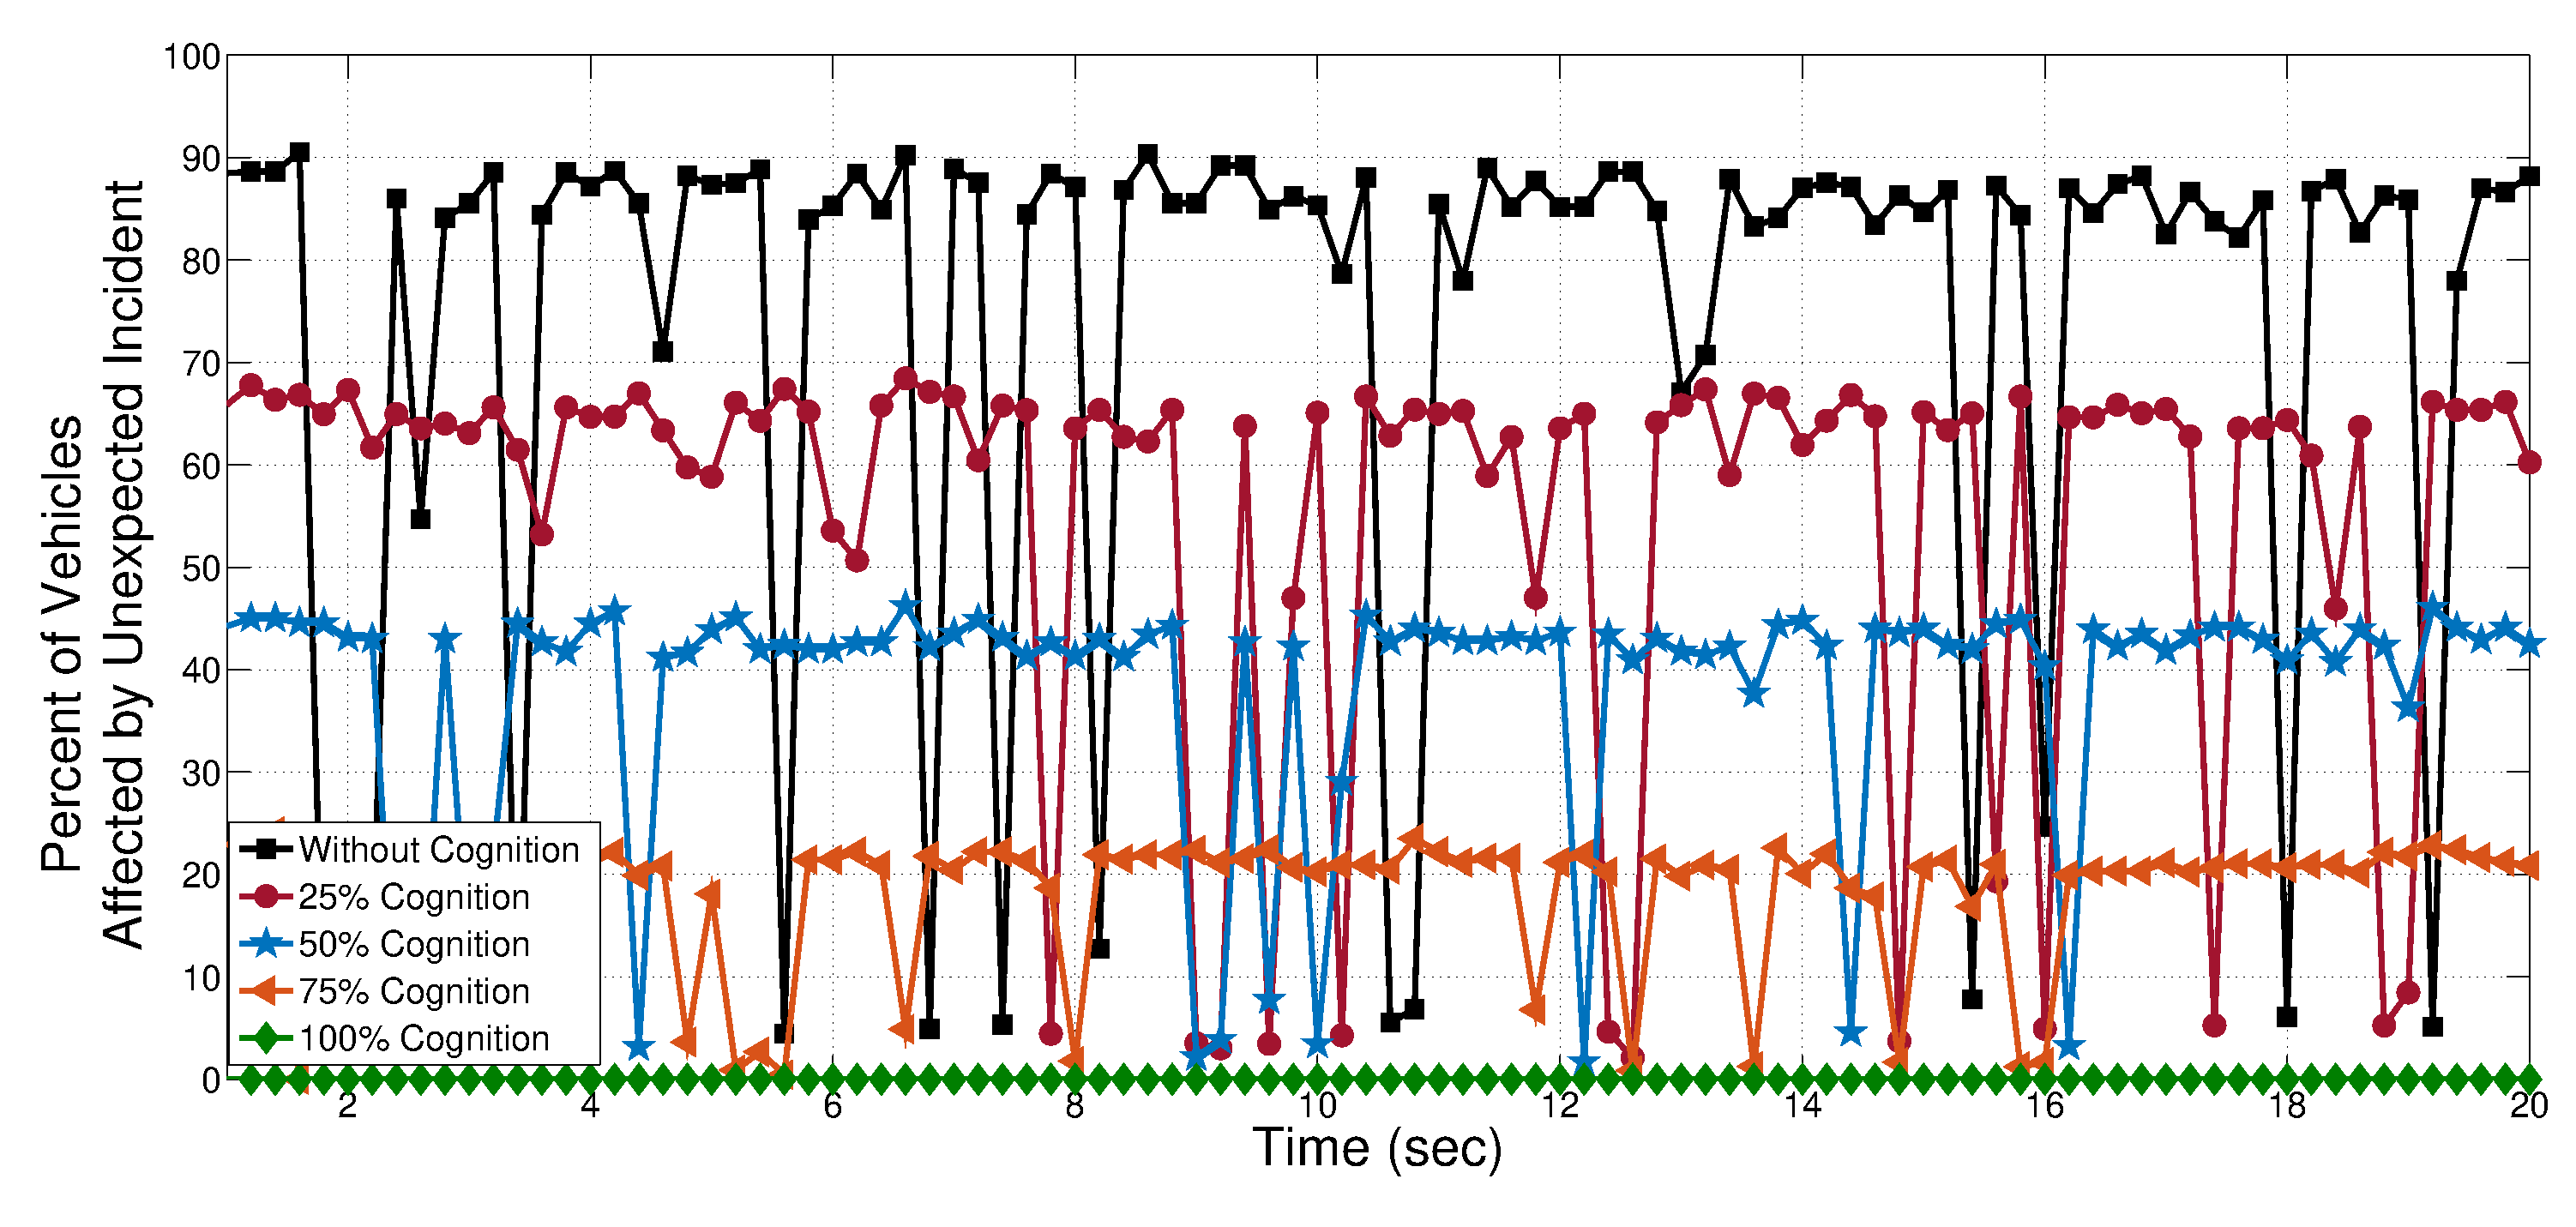
\includegraphics[width=0.47\textwidth]{figs/highwayVsTime.eps}}
  \caption{\fontsize{10}{10}\selectfont {\color {red} In case of an unexpected
  incident, \textit{e.g.} accident, sudden brake, connection failure, the
  percent of vehicles in the region effected by the incident is shown. Effected
  vehicle is defined as the vehicle that needs to rashly take an action such as
  changing lane or braking suddenly with respect to the incident. The traffic
  scenarios are generated in Simulation of Urban MObility (SUMO)~\cite{sumo} on
  the topology of Newcastle upon Tyne, UK. To have a fair comparison, both
  regions have approximately 200 vehicles which are in a motion randomly in an
  area of $1km^2$. The simulation is performed for $20~sec.$ in total and the
  effected vehicles are computed every $200~ms$. The effected vehicles are
  tested for different amount of vehicles that have the proposed cognition
  framework. The vehicles that have cognition ability are not effected by the
  unexpected incidents since they can be adapted to the current conditions fast
  and reliably. Cognition framework can deal with sudden incidents more stably
  in urban scenario than highway since high speed vehicles create more dynamic
  environment conditions in highway scenario.}}
  \label{fig:effectedVeh}
  \vspace*{-6mm}
  \end{center}
\end{figure*}

In Figure~\ref{fig:errorPlot}, the crash rate shown in the blue line is based on
the data from this report without applying our proposed cognition framework in
each vehicle. The proposed cognition framework can reduce the crash rate caused
by human errors upto $80\%$. The red line in this figure indicates a significant
influence of using our proposed cognition framework, reducing the crash rate
based on the same data.

Furthermore, the proposed cognition framework decreases the amount of
information flow due to communicating vehicles' decisions rather than their raw
sensory information. Assuming each vehicle has 5 sensors,
Figure~\ref{fig:infoFlow} shows the change in amount of sensory information flow
{\color{red}needed to provide environment awareness} with respect to the size of
the connected vehicles' network. In general, for $n$ number of connected
vehicles, each vehicle sends 5 sensory information packets to $n - 1$ neighbor
vehicles. Therefore, the total number of times that the vehicles of the given
network exchange their sensory information is $5n(n-1)$. On the other hand,
using the proposed cognition framework each vehicle only need to communicate its
decisions rather than its raw sensory information. Hence, the number of
information packets exchanged for a network of $n$ connected vehicles is
$n(n-1)$. 

\begin{figure}[!t]
  \centering
  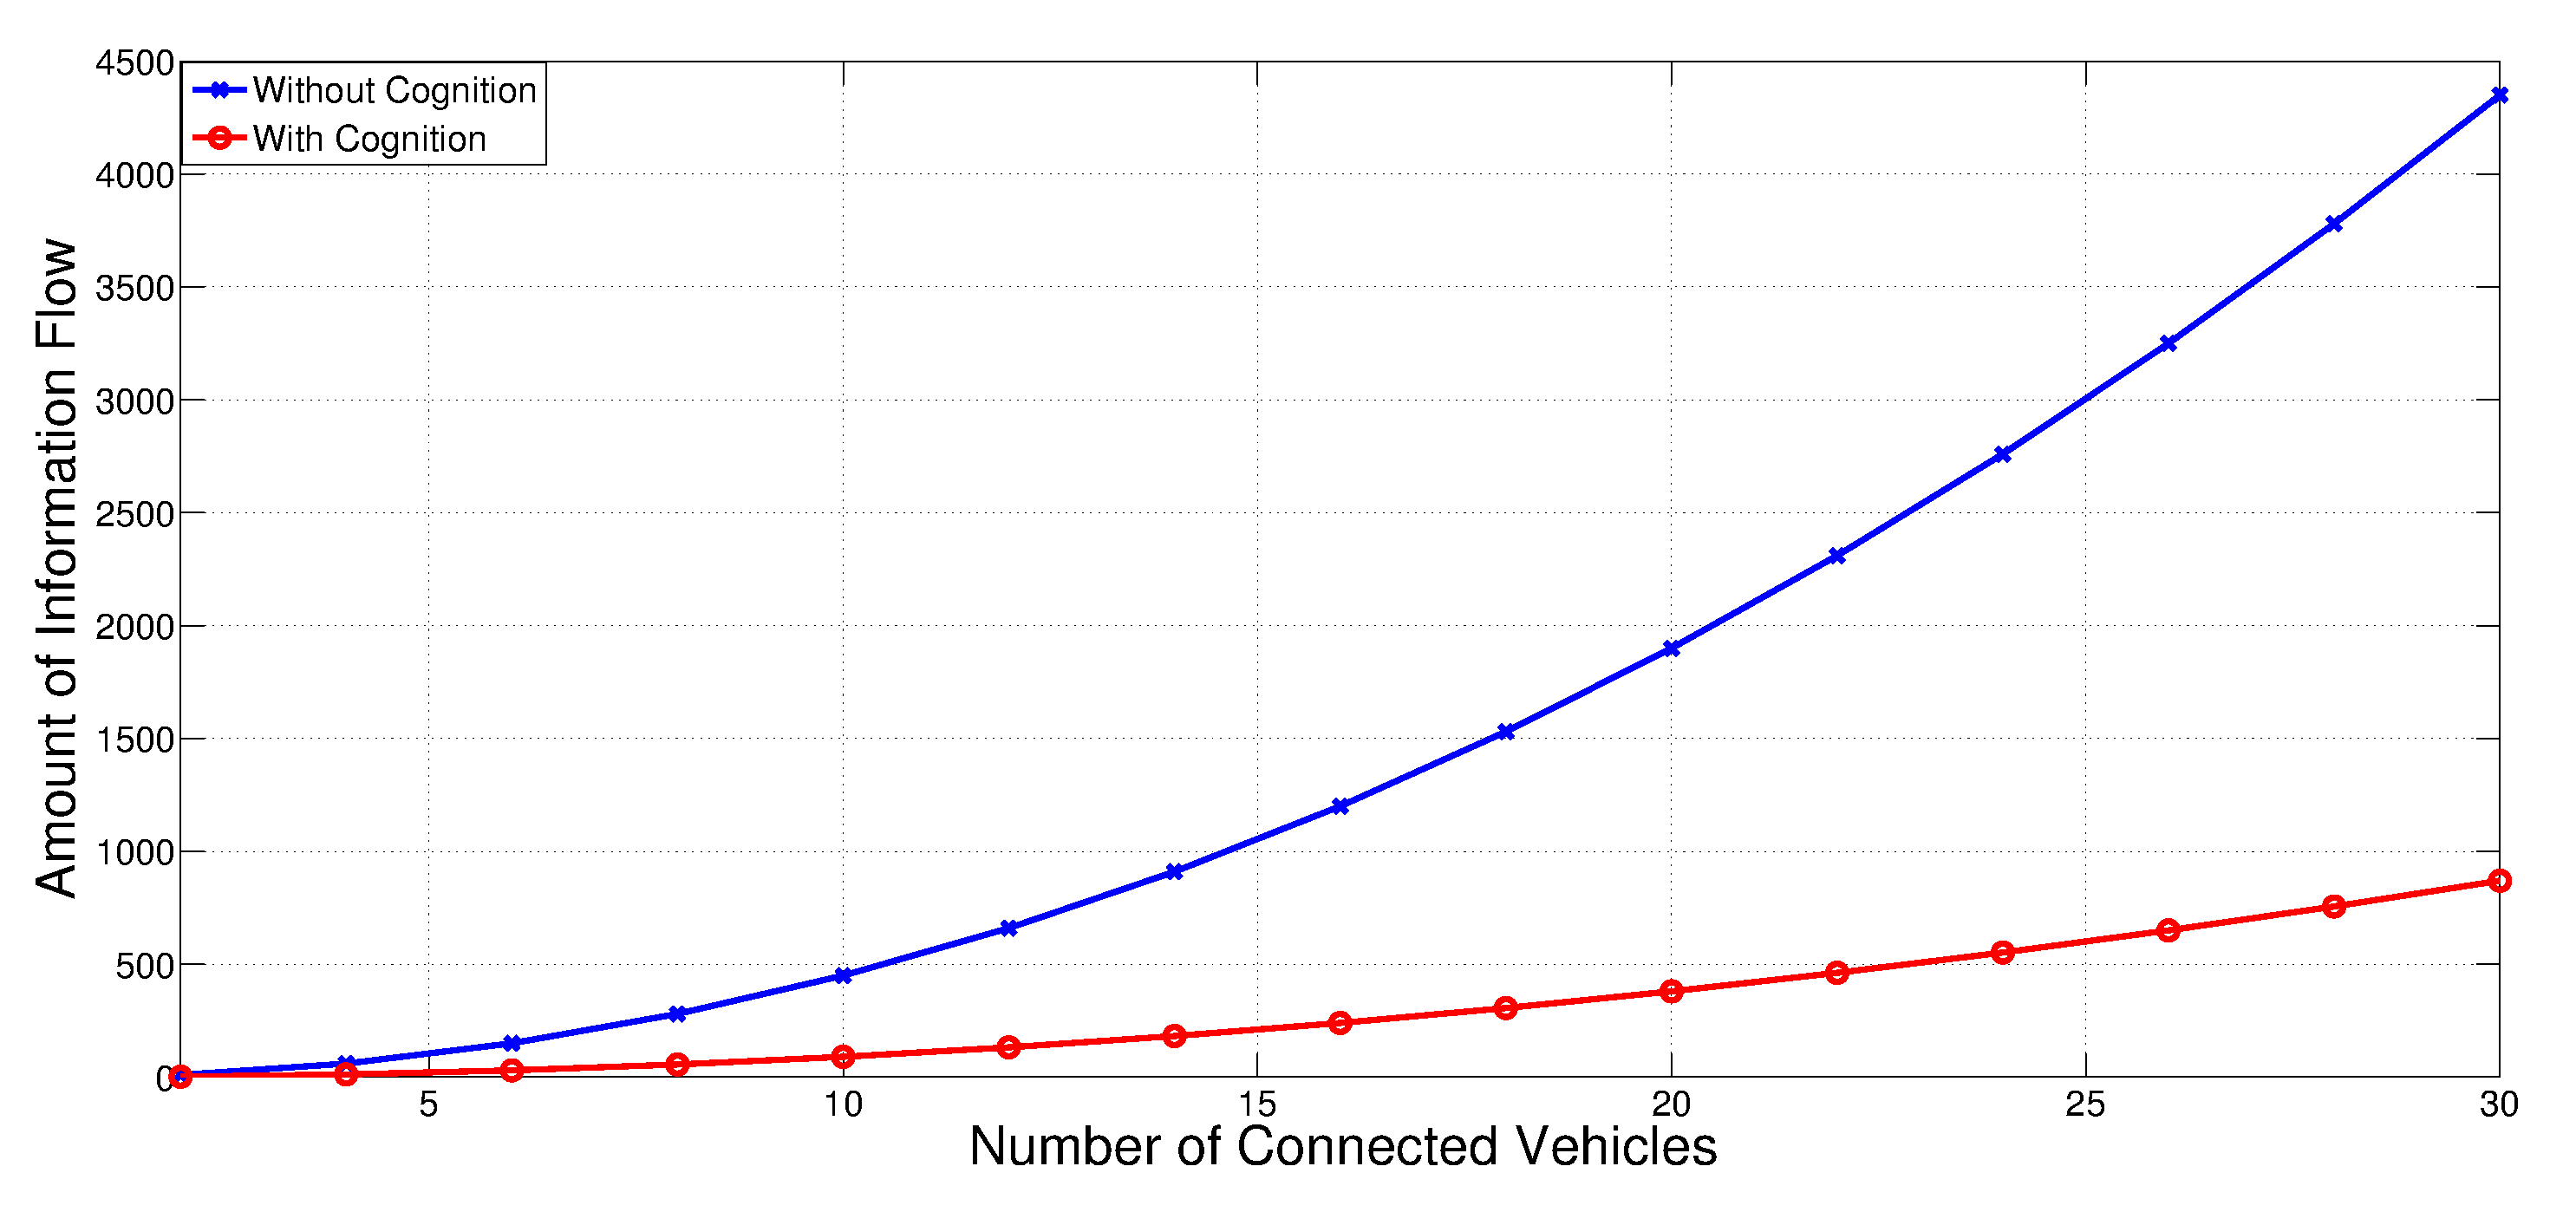
\includegraphics[width=0.49\textwidth]{figs/infoFlow.pdf}
  \caption{{\fontsize{10}{10}\selectfont The impact of cognition on the required
  data transfer rate between connected vehicles.}}
  \label{fig:infoFlow}
   \vspace*{-8mm}
\end{figure}

{\color{red} As a result, same amount of information is shared by less amount of
packet flow. Therefore, the proposed cognition framework solves the issue on the
messaging overhead. In Figure~\ref{fig:effectedVeh}, the amount of effected
vehicles in case of an unexpected incident are shown. Results show that the
amount of vehicles which need to rashly take an action with respect to the
incident is decreased by the proposed cognition framework. In
Figure~\ref{fig:urban3d}, the effect of transmission parameters on the amount of
effected vehicles in case of connection failure is shown.

The cognition framework based on AMCT provides the optimum point of Pareto
optimality on safety and comfort. The environment awareness is increased while
human-driven mistakes are minimized. The transition from half autonomous and
half human driven traffic to fully autonomous roads is operated without any
integration issue. Consequently, the aim of safety on vehicular traffic is
solidly confirmed.}

As a result, using the proposed cognition framework provides a
solution to messaging overhead.

\begin{figure}[tbh]
  \centering
  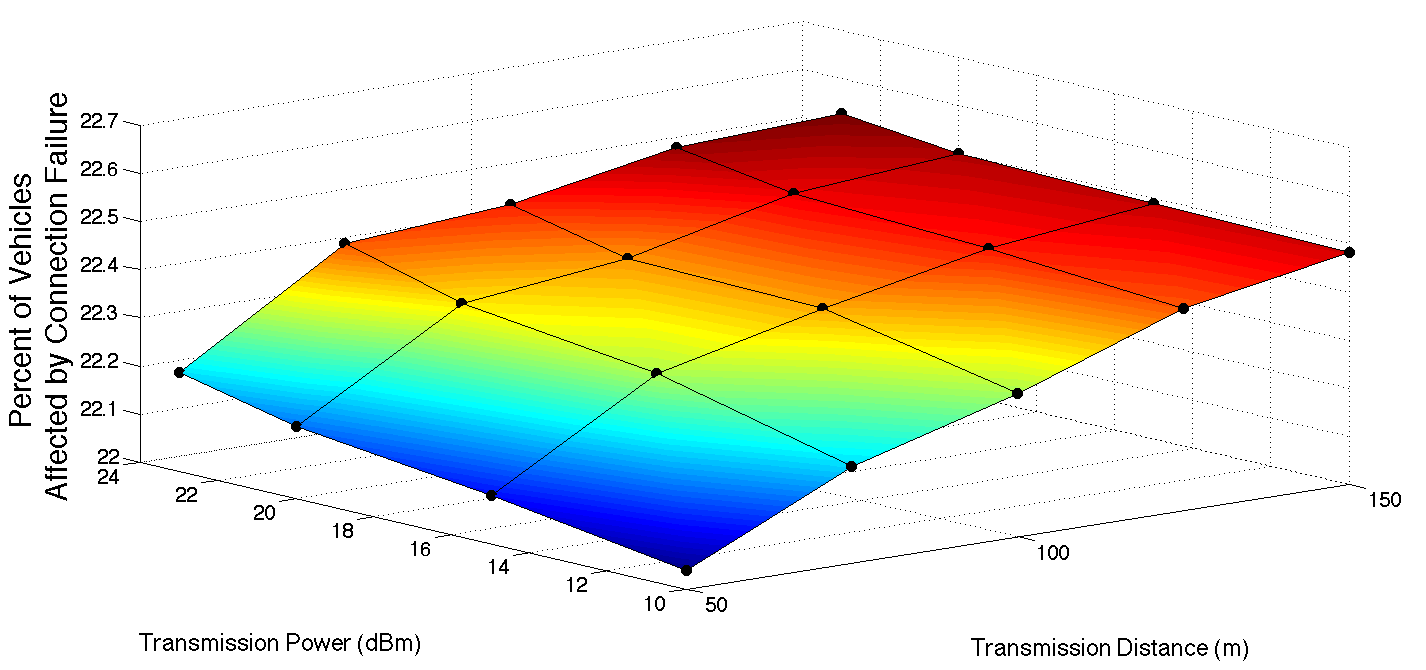
\includegraphics[width=0.5\textwidth]{figs/urban3d.png}
  \caption{{\fontsize{10}{10}\selectfont {\color {red} In case of connection
  failure with the ego vehicle and its neighbor vehicles, The percent of
  effected vehicles in the experiment region is shown with the changes of
  transmission power and distance. 75$\%$ of vehicles in chosen urban traffic
  have the cognition framework. Since The ego vehicle can connect to further the
  vehicles with the higher transmission power, number of neighbor vehicles also
  increases. Similarly, higher transmission distance covers more neighbor
  vehicles. Connection failure affects higher number of neighbor vehicles since
  higher levels on both of these factor increase the number of connected
  vehicles.}}}
  \label{fig:urban3d}
\end{figure}

\section{Summary and Research Directions}
\label{Sec:Conc}

The human-driven errors need to be considered for a successful transition from
conventional to fully autonomous vehicles. The proposed cognition framework
promises a solid decision making process to deal with this transition in
transportation system. Affective Motivational Collaboration Theory provides
fundamental evaluative, motivative, and decision making processes to improve
awareness beyond sensory information. The underlying mechanisms facilitate
reactive and deliberative decisions with respect to the events in the vehicular
environments. Using the proposed cognition framework can reduce human-driven
errors, and required amount of information exchange leading to the improvement
of safety and comfort for the occupants of the connected vehicles and their
neighbors. We will employ our proposed cognition framework in our autonomous
vehicle testbed in our future works. We will benchmark the performance of our
autonomous vehicle using our cognition framework in different traffic scenarios.

\bibliographystyle{IEEEtran}
\bibliography{mshayganfar,referencesVTM}
% \bibliography{referencesVTM}
\end{document}
